%\svnInfo $Id: Ch5_2017.tex 65 2017-08-14 19:39:16Z Georg Lindgren $ 
%$
%
\chapter{Fatigue load analysis and rain-flow cycles}
\label{cha:5}
This chapter contains some elementary facts about random fatigue and
how to compute expected fatigue damage from a stochastic, stationary
load process. The commands can be found in
\verb+Chapter5.m+, taking a few seconds to run.
\section{Random fatigue}\index[xentr]{fatigue|(}
\label{sec:randomfatigue}
\subsection{Random load models}
\label{sec:loadmodels}
This chapter presents some tools from \progname ~for
analysis of random loads in order to assess random fatigue
damage. A complete list of fatigue routines can be obtained
from the help function on {\tt fatigue}. \index[xcmds]{{\tt fatigue}}

We shall assume that the load is given by one of
three possible forms:
\begin{enumerate}
\item As measurements of the stress or strain function with some given
sampling frequency in Hz. Such loads will be called measured loads
and denoted by $x(t)$, $0\le t\le T$, where $t$ is time and $T$ is the
duration of the measurements.
\item In the frequency domain (that is important in system analysis)
as a power spectrum. This means that the signal is represented by a
Fourier series
\begin{displaymath}
x(t)\approx
m + \sum_{i=1}^{[T/2]} a_i\cos(\omega_i\,t)+b_i
\sin(\omega_i\,t)
\end{displaymath}
where $\omega_i=i\cdot 2\pi/T$ are angular
frequencies,
$m$ is the mean of the signal and $a_i,b_i$ are Fourier coefficients.
The properties are summarized in a spectral density as in described in
Section~\ref{sec:freq-model-load}.
\item In the rainflow domain, i.e.\ the measured load is given in the
form of a rainflow matrix.
\end{enumerate}

We shall now review some simple means to characterize
and analyze loads which are given in any of the forms (1)--(3), and
show how to derive characteristics, important for fatigue evaluation
and testing.

We assume that the reader has some knowledge about the concept of
cycle counting, in particular rainflow cycles, and damage accumulation
using Palmgren-Miners linear damage accumulation hypotheses.
The basic definitions are given in the end of this introduction.
Another important property is the crossing spectrum $\mu(u)$, 
introduced in Section~\ref{sect2.1}, defined as the intensity of 
upcrossings of a level $u$ by $x(t)$ as a function of $u$.
\index[xentr]{crossing spectrum}

The process of damage accumulation depends only on the values
and the order of the local extremes (maxima and minima),
in the load. The sequence \index[xentr]{turning points}
of local extremes is called the \emph{sequence of turning points}.
The irregularity factor $\alpha$ \index[xentr]{irregularity factor}
measures how dense the local \index[xentr]{mean frequency}
extremes are relatively to the mean frequency $f_0$.
For a completely regular function there would be only one
local maximum between upcrossings of the mean level, giving
irregularity factor equal to one. In the other extreme case,
there are infinitely many local extremes giving irregularity factor zero.
However, if the crossing intensity $\mu(u)$ is finite, most of those
local extremes are irrelevant for the fatigue and should be
disregarded by means of some smoothing device.

A particularly useful filter is the so-called {\em rainflow filter} 
that \index[xentr]{rainflow filter}
removes all local extremes that build rainflow cycles with amplitude
smaller than a given threshold. We shall always assume that the signals
are rainflow filtered; see Section~\ref{sec:rainflowfilter}.

If more accurate predictions of fatigue life are needed, then
more detailed models are required for the sequence of turning points.
Here the Markov chain theory has shown to be particularly useful.
There are two reasons for this:
\begin{itemize}
\item the Markov models constitute a broad
class of processes that can accurately model many real loads,
\item for Markov models, the fatigue damage prediction using rainflow method
is particularly simple, \cite{Rychlik1988Rainflow} and
\cite{Johannesson1999Rainflow}.
\end{itemize}
In the simplest case, the necessary
information is the intensity of pairs of local maxima and the following
minima, summarized in
the so-called Markov matrix or min-max matrix. The dependence
between other extremes is modelled using Markov chains,
see \cite{RychlikLindgrenLin1995} and \cite{FrendahlAndRychlik1993Rainflow}.

\subsection{Damage accumulation in irregular loads}
\label{sec:fatigueprediction}
In laboratory experiments, one often subjects a specimen of a material
to a constant amplitude load, e.g.\
$L(t)= s \sin(\omega t)$,
where $s$ and $\omega$ are the constant amplitude and
frequency, and one counts the number of cycles
(periods) until the specimen breaks. The number of load cycles until failure, $N(s)$,
as well as the amplitudes $s$ are
recorded. For small amplitudes, $s<s_{\infty}$,
the fatigue life is often very large, and is set to infinity,
$N(s)\approx\infty$, i.e.\ no
damage will be observed even during an extended experiment.
The amplitude $s_{\infty}$ is called
\emph{the fatigue limit}\index[xentr]{fatigue!limit} or
\emph{the endurance limit}\index[xentr]{endurance limit}.
In practice, one often uses a simple model for the S-N curve,
also called the W{\" o}hler curve, i.e.\
the relation between \index[xentr]{W{\"o}hler curve}
the amplitude $s$ and $N(s)$,\index[xentr]{S-N curve}
\begin{equation} \label{eq:SNmodel}
   N(s)=\left\{ \begin{array}{c@{\quad}l}
        K^{-1} s^{-\beta}, & s> s_{\infty},\\
        \infty, & s\le s_{\infty},\end{array}\right.
        \end{equation}
where $K$ and $\beta$ are material dependent parameters.
Often $K$ is considered as a random variable, usually
lognormally distributed, i.e.\ with $K^{-1}=E\epsilon^{-1}$ where
$\ln E \in\mbox{N}(0,\sigma_E^2)$,
and $\epsilon$, $\beta$ are fixed constants.

For irregular loads, also called variable amplitude loads, one
often combines the S-N curve with a cycle counting method by
means of the \emph{Palmgren-Miner linear damage accumulation theory},
\index[xentr]{Palmgren-Miner rule}
to predict fatigue failure time. A cycle counting procedure is used
to form equivalent load cycles, which are used in the life prediction.

If the $k$:th cycle in an irregular load has amplitude $s_k$ then it is assumed that
it causes a damage equal to $1/N(s_k)$. The total damage at time $t$ is
then
\begin{equation} \label{eq:Damage}\index[xentr]{damage}
  D(t)=\sum_{t_k\le t}\frac{1}{N(s_k)}=K\sum_{t_k\le
  t}s_k^\beta=K D_\beta(t),
\end{equation}
where the sum contains all cycles that have been completed
up to time $t$. Then, the fatigue life time $T^f$, say, is shorter
than $t$ if the total damage at time $t$ exceeds 1, i.e.\ if $D(t)>1$.
In other words, $T^f$ is defined as the time when $D(t)$ crosses level
1 for the first time.

A very simple predictor of $T^f$ is obtained by
replacing $K = E^{-1}\epsilon$ in Eq.~(\ref{eq:Damage}) by a constant,
for example the median value of $K$, which is equal to $\epsilon$, under the
lognormal assumption.
For high cycle fatigue, the time to failure is long, more than
$10^5/f_0$, and then for stationary (and ergodic and some other mild
assumptions) loads, the damage $D_\beta(t)$ can be approximated by its mean
$E(D_\beta(t))=d_\beta\cdot t$. Here $d_\beta$ is the {\em damage intensity},
i.e.\ how much damage is accumulated per unit time. This leads to
a very simple predictor of fatigue life time, \index[xentr]{damage!intensity}
\begin{equation}
\widehat T^f=\frac{1}{\epsilon d_\beta}.
\label{eq:fatiguelifetime}
\end{equation}

\subsection{Rainflow cycles and hysteresis loops}\label{sec:CCRainflow}

The now commonly used cycle counting method is the rainflow counting,
which was introduced 1968 by Matsuishi and Endo in
\cite{MatsuishiAndEndo1968Fatigue}. It was
designed to catch both slow and rapid variations of the load by
forming cycles by pairing high maxima with low minima even if they are
separated by intermediate extremes. Each local
maximum is used as the maximum of a {\it hysteresis loop} with an
amplitude that is computed by the rainflow algorithm.
A new definition of the rainflow cycle, equivalent to the original
definition, was given 1987 by Rychlik, \cite{Rychlik1987New}.
The formal definition is also illustrated in Figure~\ref{FigRFCdef}.
\begin{defi}[Rainflow cycle]\label{textRFCdef}
      From each local maximum $M_k$
      one shall try to reach above the same level, in the backward (left) and
      forward (right) directions, with an as small downward excursion as
      possible. The minima, $m_k^-$ and $m_k^+$, on each side are identified.
      The minimum that represents the smallest deviation from the maximum
      $M_k$ is defined as the corresponding rainflow minimum $m_k^{\rfc}$.
      The $k$:th rainflow cycle is defined as $(m_k^{\rfc},M_k)$.
\end{defi}
      \index[xentr]{rainflow cycle!definition}
      
\begin{figure}
  \centering
  %\includegraphics[width=\onefigwidth]{FigRFCdefNew}
  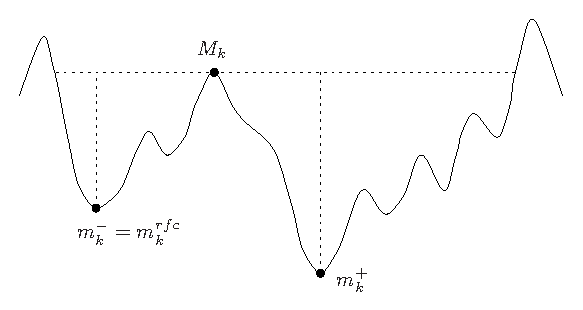
\includegraphics[width=\onefigwidth]{FigRFCdef_introNew}
  %\input{./bilder/FigRFCdef_intro.pstex_t}
\vspace{-3mm}
  \caption[Definition of the rainflow cycle as given by Rychlik]
{Definition of the rainflow cycle as given by \cite{Rychlik1987New}.
      }
  \label{FigRFCdef}
\end{figure}

If $t_k$ is the time of the $k$:th local maximum and the corresponding
rainflow amplitude is $s_k^{\rfc} = M_k - m_k^{\rfc}$, i.e.\
the amplitude of the
attached hysteresis loop, then the total damage at time $t$ is
\begin{equation} \label{eq:rainflowDamage}\index[xentr]{damage!rainflow}
  D(t)=\sum_{t_k\le t}\frac{1}{N(s_k^{\rfc})}=K\sum_{t_k\le
  t}(s_k^{\rfc})^\beta=K D_\beta(t),
\end{equation}
where the sum contains all rainflow cycles that have been completed
up to time $t$.

To use Eq.~(\ref{eq:fatiguelifetime}) to predict the fatigue life we need
the damage intensity $d_\beta$, i.e.\ the damage per time unit caused
by the rainflow cycles. If there are on the average $f_0$
maxima\footnote{We have defined $f_0$ as the mean level upcrossing
frequency, i.e.\ the mean number of times per time unit that the
load upcrosses the mean level. Thus there are in fact at least $f_0$
local maxima per time unit.  Since the rainflow filter reduces the number
of cycles, we let $f_0$ here be {\it defined as} the average number of
rainflow cycles per time unit.}
per time unit, after rainflow filtering,
and equally many rainflow cycles, and each rainflow cycle
causes an expected damage $\epsilon E(1/N_{S^{\rfc}})$
it is clear that the damage intensity is equal to
$$
d_\beta = {f_0}\, E\left((S^{\rfc})^\beta \right).
$$
Thus, an important parameter for prediction of fatigue life is the
distribution of the rainflow amplitudes and in particular the expected
value of the rainflow amplitudes raised to the material dependent
power parameter $\beta$. \progname{} contains a number
of routines for handling the rainflow cycles in observed load data
and in theoretical load models. \index[xentr]{fatigue|)}

\section{Load cycle characteristics}
\label{sec:loadcycle}

\subsection{Rainflow filtered load data}
\label{sec:rainflowfilter}

In  previous chapters we have presented models for sea wave data,
treated as functions of time. The models can be used in response
analysis for marine structures to wave forces or to compute wave
characteristics for specified random wave models, e.g.\ those defined
by their power spectrum.
%In particular, Gaussian models are very
%convenient as input to linear filters, since the output is again a
%Gaussian process with easily computable power spectral density function.

Measured wave or load signals are often very noisy and need to be smoothed
before further analysis. A common practice is to use a bandpass
filters to exclude high frequencies from the power spectrum and to
filter out slow trends. If the function is modelled by a transformed
Gaussian process {\tt xx},
as described in Section~\ref{ss:transformedGaussianmodels},
such a filtration is performed on the
inverse transformed signal {\tt yy = g(xx)}. Obviously, one should
not over-smooth data since that will affect the height of extreme
waves or cycles. Consequently, if the signal is still too irregular even after
smoothing, this is an indication that one should use the trough-to-crest
wave concept, defined as in Table~\ref{tab3_1}, instead of the simpler
min-to-max cycles. Chapter~\ref{cha:4} of this tutorial was aimed
at showing how one can compute the crest-to-trough wave
characteristics from a Gaussian or transformed Gaussian model.

The trough-to-crest cycle concept is a nonlinear means to remove small
irregularities from a load series. Another nonlinear method to remove
small cycles from data is the rainflow filtering, introduced in
\cite{Rychlik1995Simulation}, %IRk95},
and included in the \progname{} toolbox. For completeness, we describe
the algorithm of the rainflow filter.

In this tutorial we have used a simple definition of rainflow
cycles that is convenient for functions with finitely many local maxima and
minima. However, rainflow filters and rainflow cycles can be defined
for very irregular functions, like a sample function of Brownian
motion, where there are infinitely many local extremes in any finite
interval, regardless how small. This is accomplished by defining the rainflow
minimum $m^{\rfc}(t)$ for all time points $t$ of a function $x(t)$ in such a
way that the rainflow amplitude $x(t)-m^{\rfc}(t)$ is zero if the
point $x(t)$ is not a strict local maximum of the function; see
\cite{Rychlik1995Simulation} for more detailed discussion. Now, a {\it rainflow
filter with threshold $h$}, extracts all rainflow cycles
$(m^{\rfc}(t), x(t))$ such that $x(t)-m^{\rfc}(t)>h$.
Consequently, if $h<0$ then the signal is unchanged by the filter,
if $h=0$ we obtain a sequence of turning points, and, finally,
if $h>0$,  all small oscillations are removed, see Figure~\ref{fig6-1}
for an example.

\subsection{Oscillation count and the rainflow matrix}
\label{sec:oscillationcount}

The rainflow count is a generalization of the crossing count. The crossing
spectrum counts the number of times a signal upcrosses any level $u$. More
important for fatigue damage is the \index[xentr]{rainflow!count}
\emph{oscillation count}\index[xentr]{oscillation!count},
$N^{\osc}(u,v)$ that counts the number of times a signal upcrosses
an interval $[u,v]$. The oscillation count is thus a function of two
variables, $u$ and $v$, and is plotted as a bivariate count. The oscillation
count is a counting distribution for the rainflow cycles.
Consequently, if the matrix {\tt Nosc} with elements
$N^{\osc}(u_j,u_i)$ is known, for a discrete set of levels,
$u_1 \leq u_2 \leq \ldots \leq u_n$, we can compute the frequency (or rather
histogram) matrix of the rainflow count by means of the
\progname{-function}
{\tt nt2fr} and obtain the matrix {\tt Frfc = nt2fr(Nosc)}, in fatigue
practice called the {\sl rainflow matrix}\index[xentr]{rainflow matrix}.
Knowing the
rainflow matrix of a signal one can compute the oscillation
count by means of the inverse function {\tt fr2nt}.

The rainflow matrix will play an important role in the analysis
of a rainflow filtered signal. Let $x(t)$ be a measured
signal and denote by $x_h(t)$ the rainflow filtered version, filtered with
threshold $h$. Now, if we know a rainflow matrix {\tt Frfc}, say, of
$x$, then the rainflow matrix of $x_h$ is obtained by setting some
sub-diagonals of {\tt Frfc} to zero, since there are no cycles in
$x_h$ with amplitudes smaller than $h$. Thus, the oscillation
count of $x_h$ can be derived from the oscillation
count of $x$.

Note that extracting a sequence of troughs and crests
$(m_i^{\tc},M_i^{\tc})$ from the signal is closely related to rainflow
filtering. Given a reference level $u^{\tc}$, the sequence
$(m_i^{\tc},M_i^{\tc})$ can be obtained by first removing all
rainflow cycles $(m_j^{\rfc},M_j)$  such that $M_j<u^{\tc}$ or
$m_j^{\rfc}>u^{\tc}$  and then finding the min-to-max pairs in the filtered
signal.

Clearly, the oscillation count is an important characteristic
of irregularity of a sea level function, and similarly,
the expected oscillation
count, also called an
\emph{oscillation intensity matrix}, \index[xentr]{oscillation!intensity}
is an important
characteristic of the random processes used as a model for the data.
Consequently we face two
problems: how to compute the oscillation intensity for a
specified model, and if knowing the oscillation intensity,
how can one find an explicit and easy way to handle random processes with
this intensity. Note that by solving these two problems one
increases the applicability of rainflow filters considerably.
Since then, given a random process, one can find its oscillation intensity,
and next one can compute the oscillation intensity
of the rainflow filtered random process, and finally, find
a random process model for the filtered signal.

\subsection{Markov chain of turning points,
Markov matrix}\label{subsec:markov_chain}
\index[xentr]{Markov!chain}
An upcrossing of an interval $[u, v]$ occurs if the process, after an
upcrossing of the level $u$, passes the higher level $v$ before it
returns below $u$. Therefore, the oscillation intensity is closely
related to a special first passage
problem, and it can be practically handled if some Markov structure
of the process is assumed. While Gaussian processes are an important
class of models for linear filtering, Markov processes are the
appropriate models as far as rainflow filtering is concerned. In this
section a class of models, the so called Markov chain of turnings
points will be introduced.

For any load sequence we shall denote by {\tt TP} the sequence of turning
points. The sequence {\tt TP} will be called a {\em Markov chain of
turning points} if it forms a Markov chain, i.e.\ if the distribution of a
local extremum, given all previous extrema,
depends only on the value and type (minimum or maximum)
of the most recent previous extremum. The
elements in the histogram matrix of min-to-max cycles and max-to-min cycles
are equal to the observed number of transitions from a minimum
(maximum) to a maximum (minimum) of specified height.
Consequently, the probabilistic structure of the Markov chain of
turning points is fully defined by the expected histogram matrix of
min-to-max and max-to-min cycles; sometimes called
{\sl Markov matrices}\index[xentr]{Markov!matrix}. Note
that for a transformed Gaussian process, a Markov matrix for min-to-max
cycles was computed in Section~\ref{sect3_5} by
means of the \progname{} function {\tt spec2mmtpdf}. In \progname{}
there is also an older
version of that program, called {\tt spec2cmat}, which we shall use in
this chapter. The max-to-min matrix is
obtained by symmetry.\index[xcmds]{{\tt spec2mmtpdf}}

Next, the function
{\tt mctp2tc}\index[xcmds]{{\tt mctp2tc}}
(= Markov Chain of Turning Points to Trough Crests),
computes the trough2crest intensity,
using a Markov matrix to approximate the
sequence of turning points by a  Markov chain. This approximation
method is called the {\sl Markov method}. Be aware that the Markov matrix
is not the transition matrix of the Markov chain of turning points, but
the intensity of different pairs of turning points.

Figure~\ref{fig:TP_Matrix} shows the general principle of a Markov
transition count between turning points of local maxima and minima.
The values have been discretized to levels labeled {\tt 1, ..., n}, from
smallest to largest.
\begin{figure}
  % Figuren är ritad i xfig och konverteras med kommandot
  % fig2pstex fig/FigTP_Matrix
  \centering
%    \resizebox{!}{60mm}{\input{fig/FigTP_Matrix.pstex_t}}
%    \resizebox{\figwidthA}{!}{\input{fig/FigTP_Matrix.pstex_t}}
%   \input{./bilder/FigTP_Matrix.pstex_t}
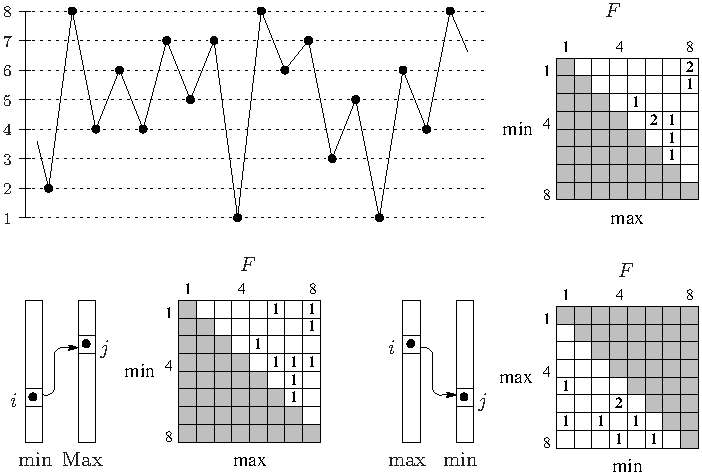
\includegraphics[width=\onefigwidth]{FigTP_MatrixNew}
\vspace{-3mm}
  \caption[General principle of a Markov
transition count]{
Part of a discrete load process where turning points are
      marked with $\bullet$. The scale to the left is the discrete levels.
      The transitions from minimum to maximum and from
      maximum to minimum are collected in the min-max matrix,
      $\bfm{F}$ and max-min matrix, $\bmh{F}$, respectively.
      The rainflow cycles are collected in the rainflow matrix,
      $\bfm{F}^{\rfc}$. The numbers in the squares are the number of observed
      cycles and the grey areas are by definition always zero.
      }
  \label{fig:TP_Matrix}
\end{figure}

Finding the expected rainflow matrix is a difficult problem and explicit
results are known only for special classes of processes, e.g.\ if {\tt x}
is a stationary diffusion, a Markov chain or a function of a vector
valued Markov chain. Markov chains are very useful in wave
analysis
since they form a broad class of processes and for several sea level
data, as well as for transformed Gaussian processes, one can  observe a
very good agreement between the observed or simulated rainflow matrix and
that computed by means of the Markov method. Furthermore, Markov
chains can be simulated in a very efficient way. However, the most important
property is that, given a rainflow matrix or oscillation
count of a Markov chain of turning points one can find its
Markov matrix. This means that a Markov chain of turning points can
be defined by either a Markov matrix {\tt FmM} or by its rainflow matrix
{\tt Frfc}, and these are connected by the following nonlinear equation
\begin{equation}
\mbox{\tt Frfc} = \mbox{\tt FmM} + {\cal F}(\mbox{\tt FmM}),
\label{eq:rfc_mM_transformation}
\end{equation}
where ${\cal F}$ is a matrix valued function, defined in
\cite{Rychlik1995Simulation},
where also an algorithm to compute the inverse $({\cal I} + {\cal F})^{-1}$ is
given. The \progname{} functions for computing {\tt Frfc} from
{\tt FmM} are {\tt mctp2rfm}\index[xcmds]{{\tt mctp2rfm}}
and {\tt mctp2rfc},\index[xcmds]{{\tt mctp2rfc}}
while the
inverse, i.e.\  {\tt FmM} as a function of  {\tt Frfc},
is computed by {\tt arfm2mctp}\index[xcmds]{{\tt arfm2mctp}}.
It might be a good idea to check the modules {\tt cycles} and
{\tt trgauss} in \progname{}
for different routines for handling these matrices.
\index[xcmds]{{\tt cycles}}\index[xcmds]{{\tt trgauss}}

\section{Cycle analysis with \progname}
\label{sec:cycleanalysiswithWAFO}\index[xentr]{cycle analysis}

In this section we shall demonstrate how \progname{} can be used to extract
rainflow cycles from a load sequence, and how the corresponding
fatigue life can be estimated.
The Markov method is used for simulation and approximation of real
load sequences. We shall use three load examples, the deep water sea
load, a simulated transformed Gaussian model, and a load sequence
generated from a special Markov structure.

\subsection{Crossing intensity}
\label{sec:crossingintensity}\index[xentr]{crossing intensity!estimation from data}
Basic to the analysis is the crossing intensity function $\mu(u)$, i.e.\
the number of times per time unit that the load up-crosses the level $u$,
considered as a function of $u$.
We illustrate the computations on the deep water sea waves data.
{\small\begin{verbatim}
      xx_sea = load('sea.dat');
      tp_sea = dat2tp(xx_sea);
      lc_sea = tp2lc(tp_sea);
      T_sea = xx_sea(end,1)-xx_sea(1,1);
      lc_sea(:,2) = lc_sea(:,2)/T_sea;
      subplot(221), plot(lc_sea(:,1),lc_sea(:,2))
      title('Crossing intensity, (u, \mu(u))')
      subplot(222), semilogx(lc_sea(:,2),lc_sea(:,1))
      title('Crossing intensity, (log \mu(u), u)')
\end{verbatim}}
\noindent
The routines {\tt dat2tp}\index[xcmds]{{\tt dat2tp}}
and {\tt tp2lc}\index[xcmds]{{\tt tp2lc}} take a load sequence and extracts
the turning points, and from this calculates the number of up-crossings
as a function of level. The plots produced, Figure~\ref{fig_wafo_6.12}, show
the crossing intensity plotted in two common modes, lin-lin of $(u, \mu(u))$
and log-lin of $(\log \mu (u), u)$.
\begin{figure}
%\centerline{%%\psfig{figure=./bilder/fig_wafo_6.12.eps,width=90mm}}
\centering
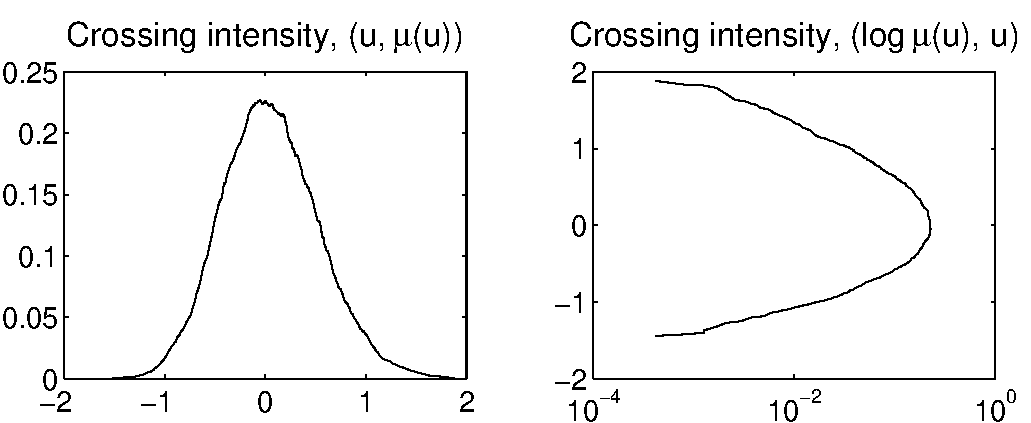
\includegraphics[width=\onefigwidth]{fatigue_3}
\vspace{-3mm}
\caption{Level crossing intensity for {\tt sea.dat}}
\label{fig_wafo_6.12}
\end{figure}

We shall also have use for the {\it mean frequency} $f_0$, i.e.\ the number of
mean level upcrossings per time unit, and the irregularity factor, $\alpha$,
which is the mean frequency divided by the mean number of local maxima per
time unit. Thus $1/\alpha$ is the average number of local maxima that occur
between the mean level upcrossings. \index[xentr]{mean frequency}
\index[xentr]{irreularity factor}

To compute $f_0$ we use the \ML{} function
{\tt interp1}, (make help {\tt interp1}), to find the crossing intensity
of the mean level.
{\small\begin{verbatim}
      m_sea = mean(xx_sea(:,2));
      f0_sea = interp1(lc_sea(:,1),lc_sea(:,2),m_sea,'linear')
      extr_sea = length(tp_sea)/(2*T_sea);
      alfa_sea = f0_sea/extr_sea
\end{verbatim}}

\subsection{Extraction of rainflow cycles}
\label{sec:rainflowextraction}\index[xentr]{rainflow cycle!computation}

We start by a study of rainflow cycles in the deep water sea data.
Recall the  definition of rainflow and min-max cycle counts.
The demo program \verb|democc| illustrates these definitions.
To use it to identify the first few rainflow and
min-max cycles, just use,
{\small\begin{verbatim}
      proc = xx_sea(1:500,:);
      democc
\end{verbatim}} \index[xcmds]{{\tt democc}}

Two windows will appear. In Demonstration Window 1, first mark the
turning points by the button TP. Then choose a local maximum (with the
buttons marked $+1,-1,+5,-5$) and find
the corresponding cycle counts, using the buttons RFC, PT. The cycles
are visualized in the other window.

We shall now examine cycle counts in the load {\tt xx\_\,sea}.
From the sequence of turning points \verb|tp| we find the rainflow
and min-max cycles in the data set,
{\small\begin{verbatim}
      RFC_sea = tp2rfc(tp_sea);
      mM_sea = tp2mm(tp_sea);
\end{verbatim}} \index[xcmds]{{\tt tp2rfc}}\index[xcmds]{{\tt tp2mm}}
Since each cycle is a pair of a local maximum and a local minimum in the
load, a cycle count can be visualized as a set of pairs in the
$\mathbb{R}^2$-plane. This is done by
the routine \verb+ccplot+. \index[xcmds]{{\tt ccplot}}
Compare the rainflow and min-max counts in the load in
Figure~\ref{fig_wafo_6.4} obtained by the following commands.
{\small \begin{verbatim}
      subplot(121), ccplot(mM_sea)
      title('min-max cycle count')
      subplot(122), ccplot(RFC_sea)
      title('Rainflow cycle count')
\end{verbatim}}

\begin{figure}
%\centerline{%%\psfig{figure=./bilder/fig_wafo_6.12.eps,width=0.9\textwidth}}
\centering 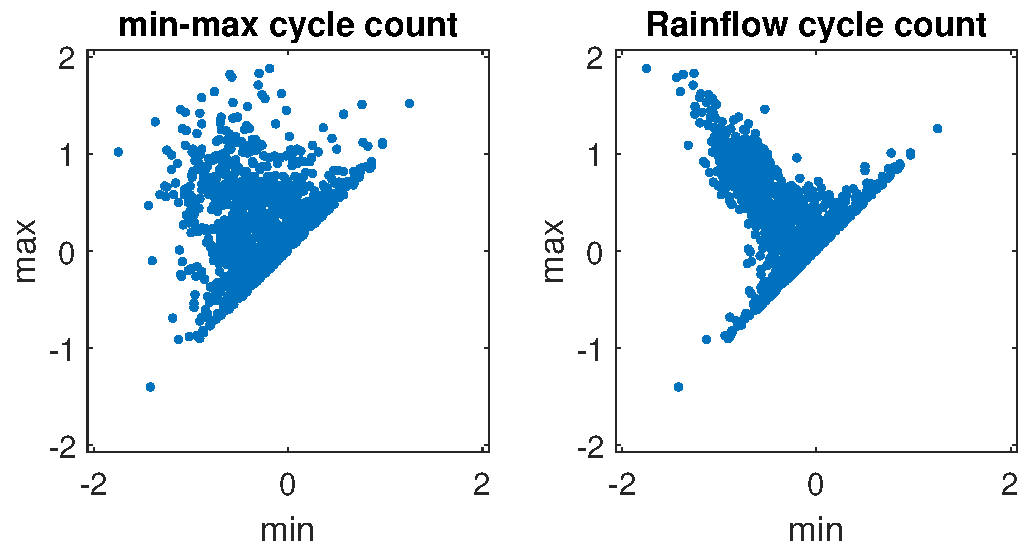
\includegraphics[width=\onefigwidth]{fatigue_4_2017}
\vspace{-3mm}
\caption[Rainflow and min-max cycle plots for {\tt sea.dat}]
{Rainflow and min-max cycle plots for {\tt sea.dat}.}
\label{fig_wafo_6.4}
\end{figure}

Observe that \verb|RFC| contains more cycles with high amplitudes,
compared to \verb|mM|. This becomes more evident in an amplitude histogram as seen in Figure~\ref{fig_wafo_6.13}.
{\small\begin{verbatim}
      ampmM_sea = cc2amp(mM_sea);
      ampRFC_sea = cc2amp(RFC_sea);
      subplot(221), hist(ampmM_sea,25);
      title('min-max amplitude distribution')
      subplot(222), hist(ampRFC_sea,25);
      title('Rainflow amplitude distribution')
\end{verbatim}}\index[xcmds]{{\tt cc2amp}}

\begin{figure}
\centering
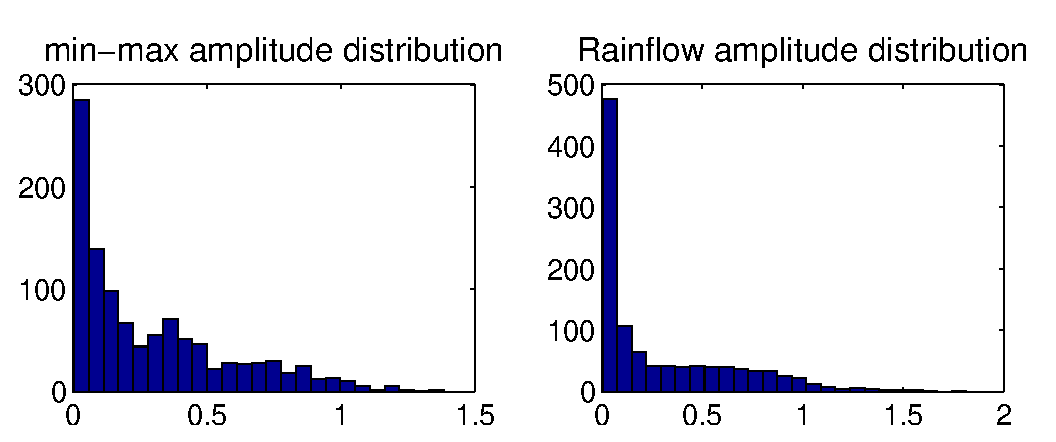
\includegraphics[width=\onefigwidth]{fatigue_5}
\vspace{-3mm}
\caption{min-max and rainflow cycle distributions for {\tt sea.dat}.}
\label{fig_wafo_6.13}
\end{figure}

\subsection{Simulation of rainflow cycles}
\label{sec:simulationcycles}\index[xentr]{simulation!of rainflow cycles}
\index[xentr]{rainflow cycle!simulation}

\subsubsection{Simulation of cycles in a Markov model}
\label{sec:simulationmarkov}
The most simple cycle model assumes that the sequence of
turning points forms a Markov chain. Then the model is completely defined
by the min-max matrix, \verb+G+. The matrix has dimension
$n \times n$, where $n$ is the number of discrete levels (e.g. $32$ or
$64$). In this example the discrete levels {\tt u} are chosen in the range
from $-1$ to $1$. The matrix {\tt G} will contain the probabilities of
transitions between the different levels in {\tt u}; see the help function
for {\tt mktestmat} for the generation of {\tt G}.
{\small\begin{verbatim}
      n = 41; param_m = [-1 1 n]; 
      u_markov = levels(param_m);
      G_markov = mktestmat(param_m,[-0.2 0.2],0.15,1);
\end{verbatim}}\index[xcmds]{{\tt mktestmat}}

%%%%%%%%%%%%%%%%%%%%%%%%%%%%%%%%%%%%%%%%%%%%%%%
% Simulation
%%%%%%%%%%%%%%%%%%%%%%%%%%%%%%%%%%%%%%%%%%%%%%%

The model is easy to simulate and this is performed by the simulation routine
\verb+mctpsim+\index[xcmds]{{\tt mctpsim}}. This routine simulates only the
sequence of turning points and not the intermediate load values.
{\small\begin{verbatim}
      T_markov = 5000;
      xxD_markov = mctpsim({G_markov []},T_markov);
      xx_markov = [(1:T_markov)' u_markov(xxD_markov)'];
\end{verbatim}}
Here \verb+xxD_markov+ takes values $1,\ldots,n$, and by changing
the scale, as in the third command line,
we get the load \verb+xx_markov+, with TP-number in first column load values between
$-1$ and 1 in second column. The first 50 samples of the simulation is plotted
in Figure~\ref{fig_wafo_6.2} by
{\small\begin{verbatim}
      plot(xx_markov(1:50,1),xx_markov(1:50,2))
\end{verbatim}}

\begin{figure}[tbh]
%\centerline{\psfig{figure=./bilder/fig_wafo_6.2.eps,width=0.9\textwidth}}
\centering
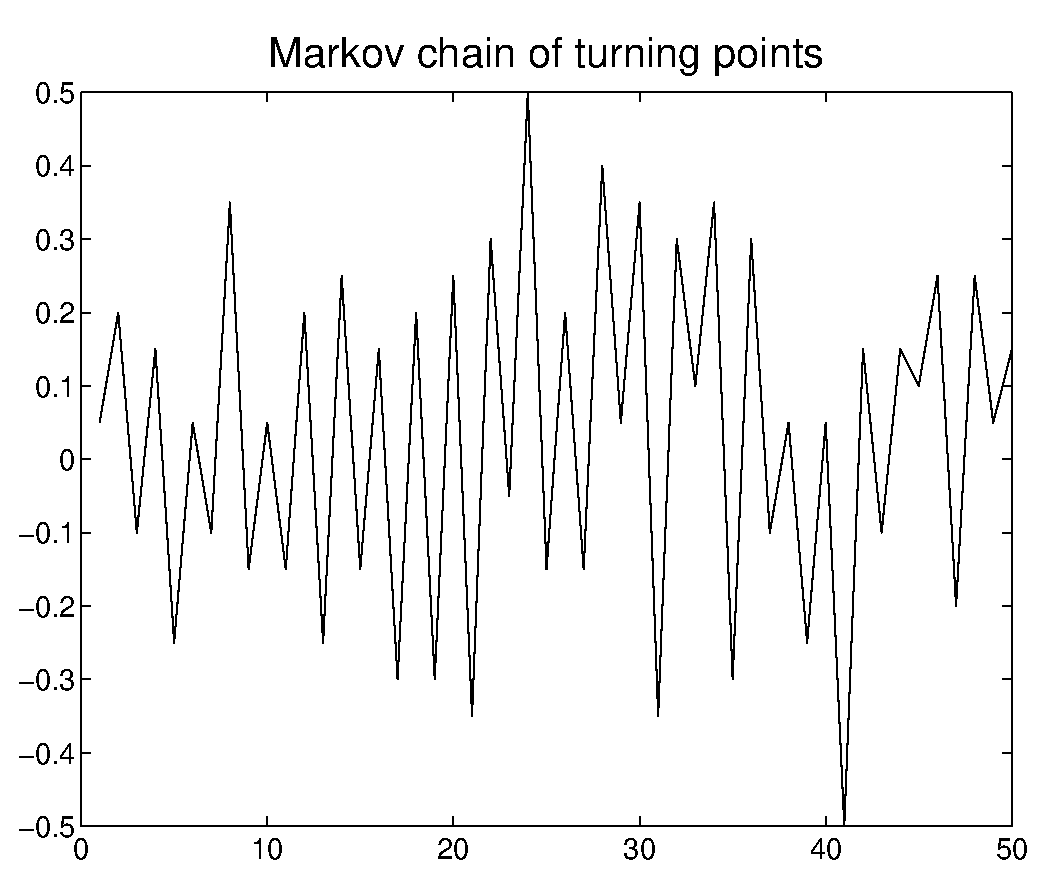
\includegraphics[width=\narrowfigwidth]{fatigue_6}
\vspace{-3mm}
\caption[Simulated Markov sequence of turning points]
{Simulated Markov sequence of turning points.}
\label{fig_wafo_6.2}
\end{figure}

We shall later use the matrix \verb+G_markov+ to calculate the
theoretical rainflow matrix, but first we construct a similar
sequence of turning points from a transformed Gaussian model.

\subsubsection{Rainflow cycles in a transformed Gaussian model}
\label{sec:RFC_filtered}
In this example we shall consider a sea-data-like series obtained as
a transformed Gaussian model with {\sc Jonswap} spectrum.
Since that \index[xentr]{Jonswap spectrum}
spectrum contains also rather high frequencies a {\sc Jonswap} load will
contain many cycles with small amplitude. These are often uninteresting
and can be removed by a rainflow filter as follows.

Let {\tt g} be the Hermite transformation proposed by Winterstein,
which we used in Chapter~\ref{cha:2}. Suppose the spectrum 
is of the {\sc Jonswap} type. To get the transform we need as input the
approximative higher moments, skewness and kurtosis, which are
automatically calculated from the spectrum by the routine
\verb+spec2skew+. We define the spectrum structure,
including the transformation, and simulate the transformed Gaussian
load \verb+xx_herm+. The routine {\tt dat2dtp}\index[xcmds]{{\tt dat2dtp}}
extracts the turning points discretized to the
levels specified by the parameter vector {\tt param}.
\index[xcmds]{{\tt spec2skew}}\index[xcmds]{{\tt hermitetr}}

Note that when calling the simulation routine
\verb+spec2sdat+\index[xcmds]{{\tt spec2sdat}} with a spectrum structure
including a transformation, the input spectrum must be normalized to have
standard deviation 1, i.e.\ one must divide the spectral values by
the variance \verb+sa^2+.
{\small
\begin{verbatim}
      me = mean(xx_sea(:,2));
      sa = std(xx_sea(:,2));
      Hm0_sea = 4*sa;
      Tp_sea = 1/max(lc_sea(:,2));
      SJ = jonswap([],[Hm0_sea Tp_sea]);

      [sk, ku] = spec2skew(SJ);
      SJ.tr = hermitetr([],[sa sk ku me]);
      param_h = [-1.5 2 51];
      SJnorm = SJ;
      SJnorm.S = SJnorm.S/sa^2;
      xx_herm = spec2sdat(SJnorm,[2^15 1],0.1);
      h = 0.2;
      [dtp,u_herm,xx_herm_1] = dat2dtp(param_h,xx_herm,h);
      plot(xx_herm(:,1),xx_herm(:,2),'k','LineWidth',2);
      hold on;
      plot(xx_herm_1(:,1),xx_herm_1(:,2),'k--','Linewidth',2);
      axis([0 50 -1 1]), hold off;
      title('Rainflow filtered wave data')
\end{verbatim}}

The rainflow filtered data \verb+xx_herm_1+ contains the turning
points of \verb+xx_herm+ with rainflow cycles less than \verb+h=0.2+
removed. In Figure~\ref{fig6-1} the dashed curve connects the
remaining turning points after filtration.

\begin{figure}[tbh]
\centering
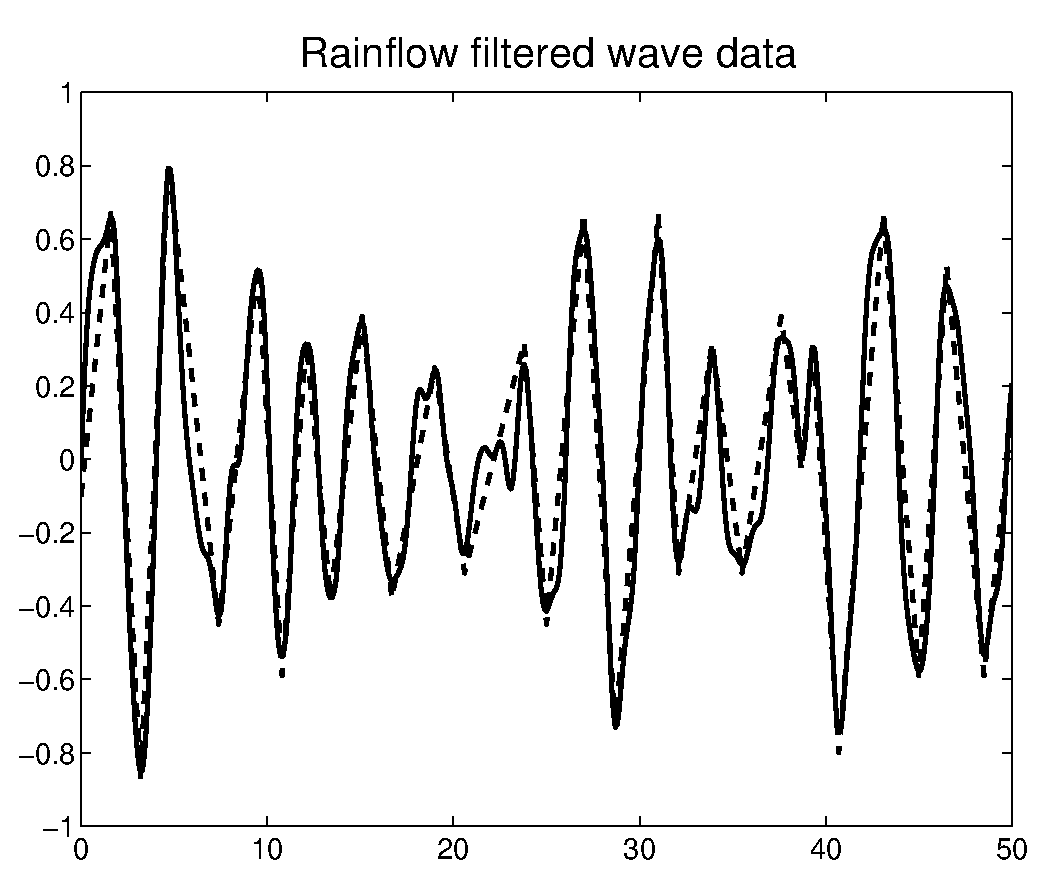
\includegraphics[width=\narrowfigwidth]{fatigue_7}
\vspace{-3mm}
\caption[Hermite transformed wave data and rainflow filtered turning points]{
Hermite transformed wave data together with rainflow filtered turning
  points, {\tt h = 0.2}.}
\label{fig6-1}
\end{figure}

Try different degree of filtering on the Ochi transformed sequence and
see how it affects the min-max cycle distribution. You can use the
following sequence of commands, with different \verb+h+ -values;
see Figure~\ref{fig_wafo_6.16} for the results. Note that the rainflow cycles
have their original values in the left figure but that they have been
discretized to the discrete level defined by \verb+param_h+ in the
right figure.
{\small\begin{verbatim}
      tp_herm=dat2tp(xx_herm);
      RFC_herm=tp2rfc(tp_herm);
      mM_herm=tp2mm(tp_herm);
      h=0.2;
      [dtp,u,tp_herm_1]=dat2dtp(param_h,xx_herm,h);
      RFC_herm_1 = tp2rfc(tp_herm_1);
      subplot(121), ccplot(RFC_herm)
      title('h=0')
      subplot(122), ccplot(RFC_herm_1)
      title('h=0.2')
\end{verbatim}}

\begin{figure}
\centering
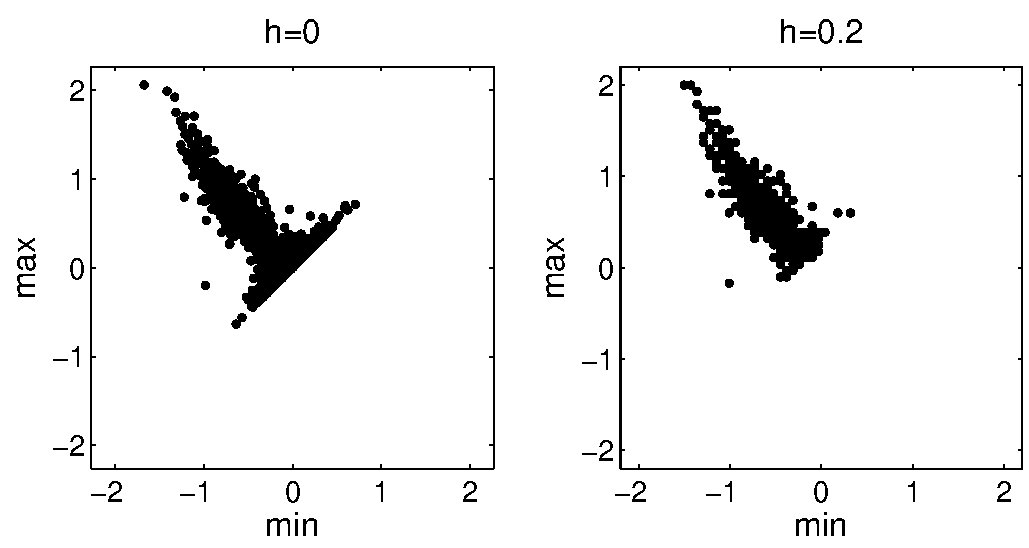
\includegraphics[width=\onefigwidth]{fatigue_8}
\vspace{-3mm}
\caption[Rainflow cycles and rainflow filtered rainflow cycles]{
Rainflow cycles and rainflow filtered rainflow cycles in
the transformed Gaussian process.}
\label{fig_wafo_6.16}
\end{figure}

%%%%%%%%%%%%%%%%%%%%%%%%%%%%%%%%%%%%%%%%%%%%%%%
% Calculating the Rainflow Matrix
%%%%%%%%%%%%%%%%%%%%%%%%%%%%%%%%%%%%%%%%%%%%%%%

\subsection{Calculating the Rainflow Matrix}
\label{sec:calrainflowmatrix}\index[xentr]{rainflow matrix!computation}

We have now shown how to extract rainflow cycles from a load
sequence and to perform rainflow filtering in measured or
simulated load sequences. Next we shall
demonstrate how the expected (theoretical) rainflow matrix can be
calculated in any random load or wave model, defined either as a
Markov chain of turning points, or as a stationary random process
with some spectral density.
We do this by means of the Markov method based on the max-min
transition matrix for the sequence of turning points.
This matrix can either be directly estimated from
or assigned to a load sequence, or it can be calculated from the
correlation or spectrum structure of a transformed Gaussian model
by the methods described in Section~\ref{sect3_5}.

\subsubsection{Calculation of rainflow matrix in the Markov model}
\label{sec:calrfcmatrixinmarkovmodel}

The theoretical rainflow matrix \verb+Grfc+ for the Markov model is
calculated in \progname{} by the routine
\verb+mctp2rfm+\index[xcmds]{{\tt mctp2rfm}}.
Let \verb+G_markov+ be as in Section~\ref{sec:simulationmarkov} and
calculate the theoretical rainflow matrix by
{\small\begin{verbatim}
      Grfc_markov=mctp2rfm({G_markov []});
\end{verbatim}}

A cycle matrix, e.g.\ a min-max or rainflow matrix, can be
plotted by \verb+cmatplot+\index[xcmds]{{\tt cmatplot}}.
Now we will compare the min-max and the rainflow matrices.
{\small\begin{verbatim}
      subplot(121),cmatplot(u_markov,u_markov,G_markov),...
              axis('square')
      subplot(122),cmatplot(u_markov,u_markov,Grfc_markov),...
              axis('square')
\end{verbatim}}
Both 2D- and 3D-plots can be drawn;
see the help on \verb+cmatplot+. 
It is also possible to plot many matrices in one call.
{\small\begin{verbatim}
      cmatplot(u_markov,u_markov,{G_markov Grfc_markov},3)
\end{verbatim}}

A plot with \verb+method = 4+ gives contour lines;
see Figure~\ref{fig_wafo_6.1}.
Note that for high maxima and low minima, the rainflow matrix has
a pointed shape while the min-max matrix has a more rounded shape.
{\small\begin{verbatim}
      cmatplot(u_markov,u_markov,{G_markov Grfc_markov},4)
      subplot(121), axis('square'),...
                    title('min2max transition matrix')
      subplot(122), axis('square'), title('Rainflow matrix')
\end{verbatim}}

\begin{figure}
\centering
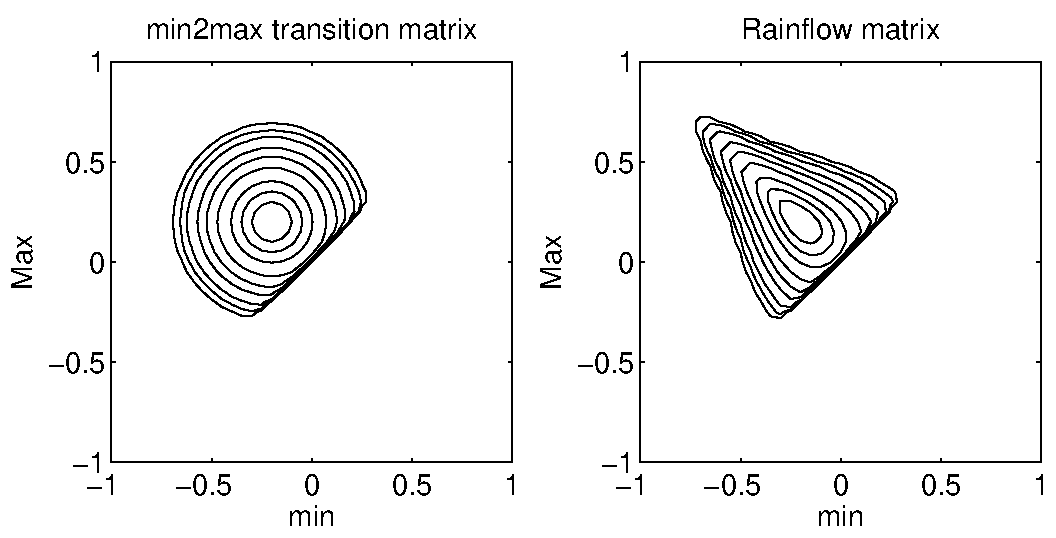
\includegraphics[width=\onefigwidth]{fatigue_9}
\vspace{-3mm}
\caption[Theoretical min-max  and
rainflow matrix for test Markov sequence]
{min-max-matrix and theoretical
rainflow matrix for test Markov sequence.}
\label{fig_wafo_6.1}
\end{figure}

We now compare the theoretical rainflow matrix with an observed rainflow
matrix obtained in the simulation. In this case we have simulated a
discrete Markov chain of turning points with states {\tt 1,...,n} and put
them in the variable \verb+xxD_markov+. It is turned into a rainflow
matrix by the  routine \verb|dtp2rfm|. 
The comparison in \index[xcmds]{{\tt dtp2rfm}} 
Figure~\ref{fig_wafo_6.3} between the observed
rainflow matrix and the theoretical one is produced as follows.
{\small\begin{verbatim}
      n = length(u_markov);
      Frfc_markov = dtp2rfm(xxD_markov,n);
      cmatplot(u_markov,u_markov,...
               {Frfc_markov Grfc_markov*T/2},3)
      subplot(121), axis('square')
                    title('Observed rainflow matrix')
      subplot(122), axis('square')
                    title('Theoretical rainflow matrix')
\end{verbatim}}

Note that in order to compare the observed matrix \verb+Frfc_markov+ 
with the theoretical matrix \verb+Grfc_markov+ we have 
to multiply the latter by the
number of cycles in the simulation which is equal to {\tt T/2}.

\begin{figure}[tbh]
\centering
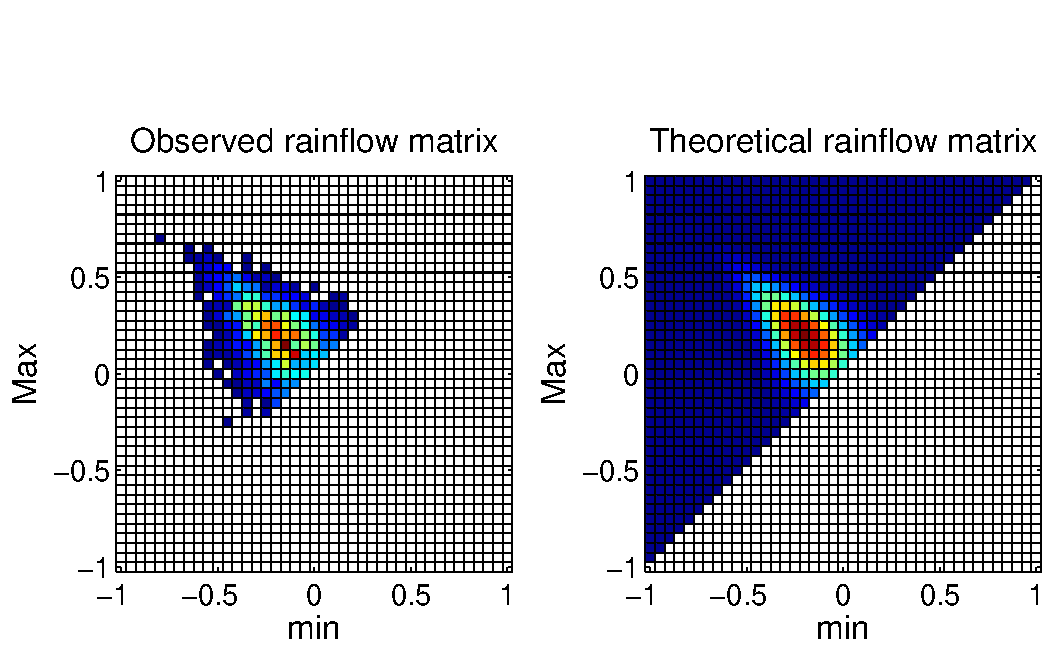
\includegraphics[width=\onefigwidth]{fatigue_10}
\vspace{-3mm}
\caption[Observed and theoretical rainflow matrix for test Markov sequence]
{Observed and theoretical rainflow matrix for test Markov sequence.}
\label{fig_wafo_6.3}
\end{figure}

We end this section by an illustration of the rainflow smoothing
operation. The observed rainflow matrix is rather irregular, due to
the statistical variation in the finite sample. 
To facilitate comparison with the theoretical
rainflow matrix we smooth it by the built in smoothing facility in the routine {\tt cc2cmat}. \index[xcmds]{{\tt cc2cmat}}
To see how it works for different
degrees of smoothing we calculate the rainflow cycles by {\tt tp2rfc}.
{\small\begin{verbatim}
      tp_markov = dat2tp(xx_markov);
      RFC_markov = tp2rfc(tp_markov);
      h = 0.2;
      Frfc_markov_smooth = cc2cmat(param_m,RFC_markov,[],1,h);
      cmatplot(u_markov,u_markov,...
               {Frfc_markov_smooth Grfc_markov*T/2},4)
      subplot(121), axis('square')
                    title('Smoothed observed rainflow matrix')
      subplot(122), axis('square')
                    title('Theoretical rainflow matrix')
\end{verbatim}}

Here, the smoothing is done as a kernel smoother with a bandwidth
parameter {\tt h = 1}. The effect of the smoothing is shown in
Figure~\ref{fig_wafo_6.7}.

\begin{figure}
\centering
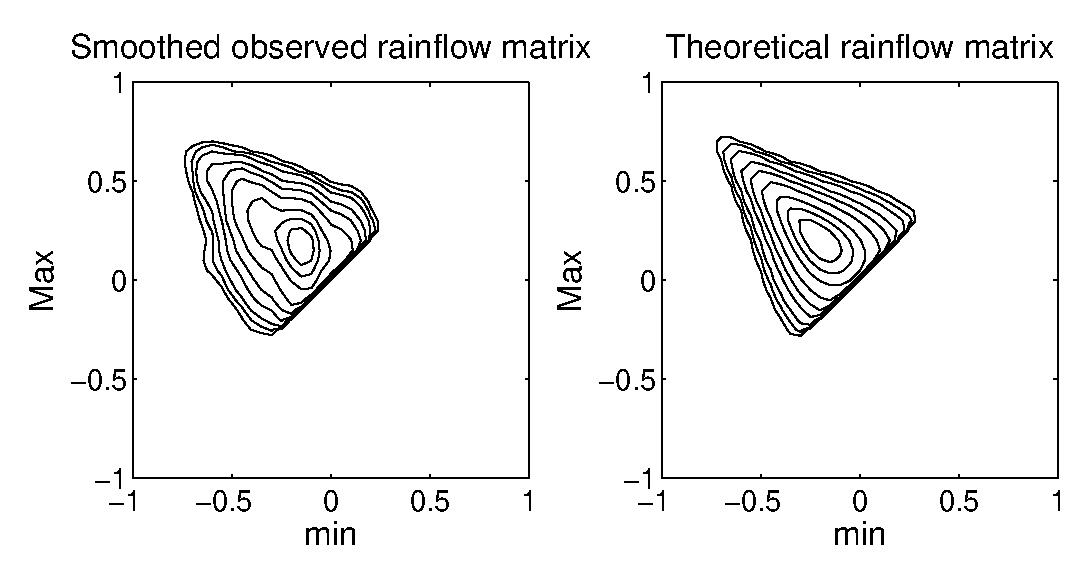
\includegraphics[width=\onefigwidth]{fatigue_11}
\vspace{-3mm}
\caption[Smoothed observed and rainflow matrix for test
  Markov sequence]
{Smoothed observed and calculated rainflow matrix for test
  Markov sequence.}
\label{fig_wafo_6.7}
\end{figure}

\subsubsection{Rainflow matrix from spectrum}
\label{sec:rainflowfromspectrum}\index[xentr]{rainflow matrix!computation}

We are now ready to demonstrate how the rainflow matrix can be calculated
in a load or wave model defined by its correlation or spectrum structure.
We chose the transformed Gaussian model with the Hermite transform
\verb+xx_herm+ which was studied in Section~\ref{sec:RFC_filtered}.
This model was defined by its {\sc Jonswap} spectrum and the standard
Hermite transform for asymmetry.

We first need to find the structure of the turning points,
which is defined by the min-to-max
density by the methods in Section~\ref{sect3_5}. We start by computing
an approximation, \verb+GmM3_herm+, of the min-max density by means of the
cycle routine {\tt spec2cmat} (as an alternative one can
use \verb+spec2mmtpdf+)\index[xcmds]{{\tt spec2cmat}}.
The type of cycle is specified
by a cycle parameter, in this case {\tt 'Mm'}.
{\small\begin{verbatim}
      GmM3_herm = spec2cmat(SJ,[],'Mm',[],param_h,2);
\end{verbatim}}
\noindent The result is seen in Figure~\ref{fig_wafo_6.5}.

Then, we approximate the distribution of the turning points by a
Markov chain with transitions between extrema calculated from
\verb+GmM3_herm+, and compute the rainflow matrix
by Eq.~(\ref{eq:rfc_mM_transformation}).
{\small\begin{verbatim}
      Grfc_herm = mctp2drfm({GmM3_herm.f,[]});
\end{verbatim}}\index[xcmds]{{\tt mctp2drfm}}
In \progname{}, the rainflow matrix can be calculated directly
from the spectrum by the cycle distribution routine {\tt spec2cmat} by
specifying the cycle parameter to {\tt 'rfc'}.
{\small\begin{verbatim}
      Grfc_direct_herm = spec2cmat(SJ,[],'rfc',[],[],2);
\end{verbatim}} \index[xcmds]{{\tt spec2cmat}}
\noindent
The output is a structure array which contains the rainflow matrix in the
cell {\tt .f}.

The min-max matrix \verb+GmM3_herm+ and the rainflow matrix
\verb+Grfc_herm+ are shown together in Figure~\ref{fig_wafo_6.5},
obtained using the following commands.
{\small\begin{verbatim}
      u_herm = levels(param_h);
      cmatplot(u_herm,u_herm,{GmM3_herm.f Grfc_herm},4)
      subplot(121), axis('square'),...
                    title('min-max matrix')
      subplot(122), axis('square'),...
                    title('Theoretical rainflow matrix')
\end{verbatim}}
\begin{figure}
  \centering
  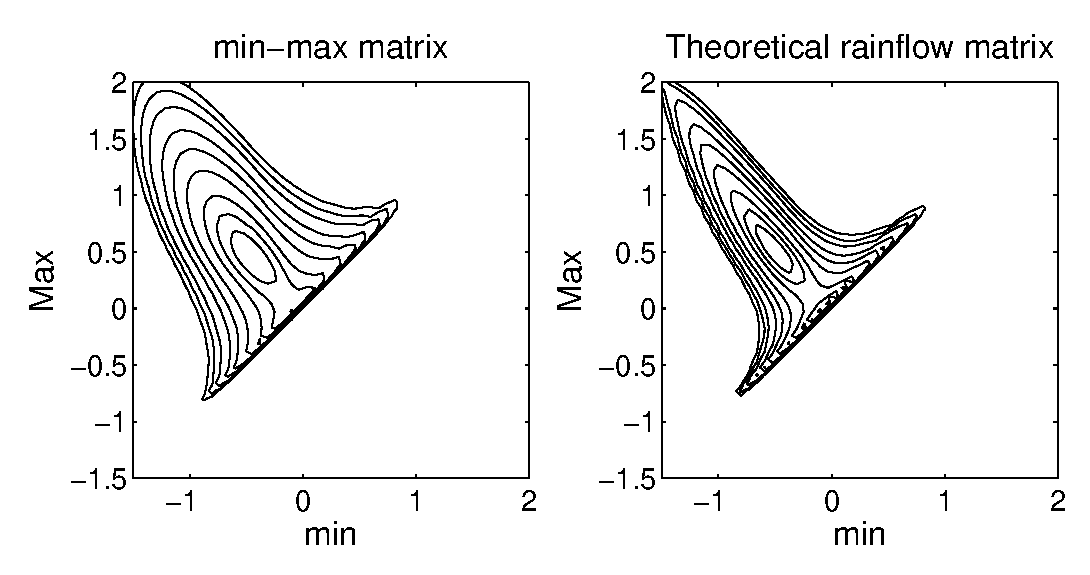
\includegraphics[width=\onefigwidth]{fatigue_12}
\vspace{-3mm}
\caption[min-max and theoretical rainflow matrix for Hermite waves]
{min-max matrix and theoretical rainflow matrix for Hermite transformed
Gaussian waves.}
\label{fig_wafo_6.5}
\end{figure}

We can also compare the theoretical min-max matrix with the observed
cycle count and the theoretical rainflow matrix with the observed
one. In both comparisons we smooth the observed matrix to get a more
regular structure. We also illustrate the multi-plotting capacity of
the routine {\tt cmatplot}\index[xcmds]{{\tt cmatplot}}.
{\small\begin{verbatim}
      tp_herm = dat2tp(xx_herm);
      RFC_herm = tp2rfc(tp_herm);
      mM_herm = tp2mm(tp_herm);
      h = 0.2;
      FmM_herm_smooth = cc2cmat(param_o,mM_herm,[],1,h);
      Frfc_herm_smooth = cc2cmat(param_o,RFC_herm,[],1,h);
      T_herm=xx_herm(end,1)-xx_herm(1,1);
      cmatplot(u_herm,u_herm,{FmM_herm_smooth ...
               GmM3_herm.f*T_herm/2;...
               Frfc_herm_smooth Grfc_herm*T_herm/2},4)
      subplot(221), axis('square')
                    title('Observed smoothed min-max matrix')
      subplot(222), axis('square')
                    title('Theoretical min-max matrix')
      subplot(223), axis('square')
                    title('Observed smoothed rainflow matrix')
      subplot(224), axis('square')
                    title('Theoretical rainflow matrix')
\end{verbatim}}
\begin{figure}
  \centering
  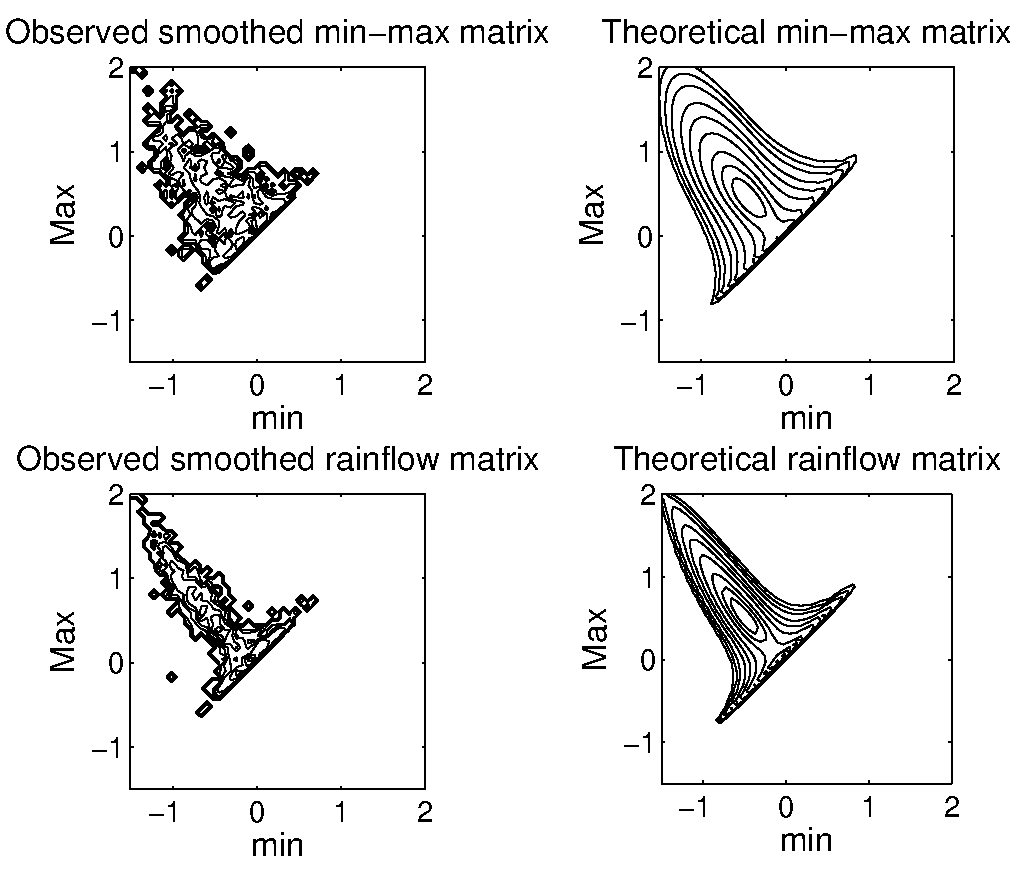
\includegraphics[width=\onefigwidth]{fatigue_13}
\vspace{-3mm}
\caption[Observed smoothed and theoretical min-max matrix]
{Observed smoothed and theoretical min-max matrix,
and observed smoothed and theoretical rainflow matrix for Hermite transformed
Gaussian waves.}
\label{fig_wafo_6.8}
\end{figure}

\subsection{Simulation from crossings structure}
\label{sec:crossingrainflowsimulation}
\index[xentr]{simulation!from crossings structure}

In fatigue experiments it is important to generate load sequences with a
prescribed rainflow or other crossing property. Besides the previously
used simulation routines for Markov loads and spectrum loads,
\progname ~contains algorithms for generation of random load sequences that
have a specified average rainflow distribution or a specified irregularity and
crossing spectrum. We illustrate the crossing structure simulation
by means of the routine {\tt lc2sdat}\index[xcmds]{{\tt lc2sdat}}.
Simulation from a rainflow distribution can be achieved by first calculating the 
corresponding Markov matrix and then simulate by means of 
{\tt mctpsim}. \index[xcmds]{{\tt mctpsim}}

The routine {\tt lc2sdat} simulates a load with specified irregularity factor \index[xentr]{irregularity factor}
and crossing spectrum. \index[xentr]{crossing spectrum}
We first estimate these quantities in the
simulated Hermite transformed Gaussian load, and then simulate series with
the same crossing spectrum but with varying irregularity factor. The sampling
variability increases with decreasing irregularity factor, as is seen in
Figure~\ref{fig_wafo_6.9}. The figures were
generated by the following commands.
{\small\begin{verbatim}
      cross_herm = dat2lc(xx_herm);
      alpha1 = 0.25;
      alpha2 = 0.75;
      xx_herm_sim1 = lc2sdat(cross_herm,500,alpha1);
      cross_herm_sim1 = dat2lc(xx_herm_sim1);
      subplot(211)
      plot(cross_herm(:,1),cross_herm(:,2)/max(cross_herm(:,2)))
      hold on
      stairs(cross_herm_sim1(:,1),...
          cross_herm_sim1(:,2)/max(cross_herm_sim1(:,2)))
      hold off
      title('Crossing intensity, \alpha = 0.25')
      subplot(212)
      plot(xx_herm_sim1(:,1),xx_herm_sim1(:,2))
      title('Simulated load, \alpha = 0.25')

      xx_herm_sim2 = lc2sdat(500,alpha2,cross_herm);
      cross_herm_sim2 = dat2lc(xx_herm_sim2);
      subplot(211)
      plot(cross_herm(:,1),cross_herm(:,2)/max(cross_herm(:,2)))
      hold on
      stairs(cross_herm_sim2(:,1),...
          cross_herm_sim2(:,2)/max(cross_herm_sim2(:,2)))
      hold off
      title('Crossing intensity, \alpha = 0.75')
      subplot(212)
      plot(xx_herm_sim2(:,1),xx_herm_sim2(:,2))
      title('Simulated load, \alpha = 0.75')
\end{verbatim}}

\begin{figure}
  \centering
  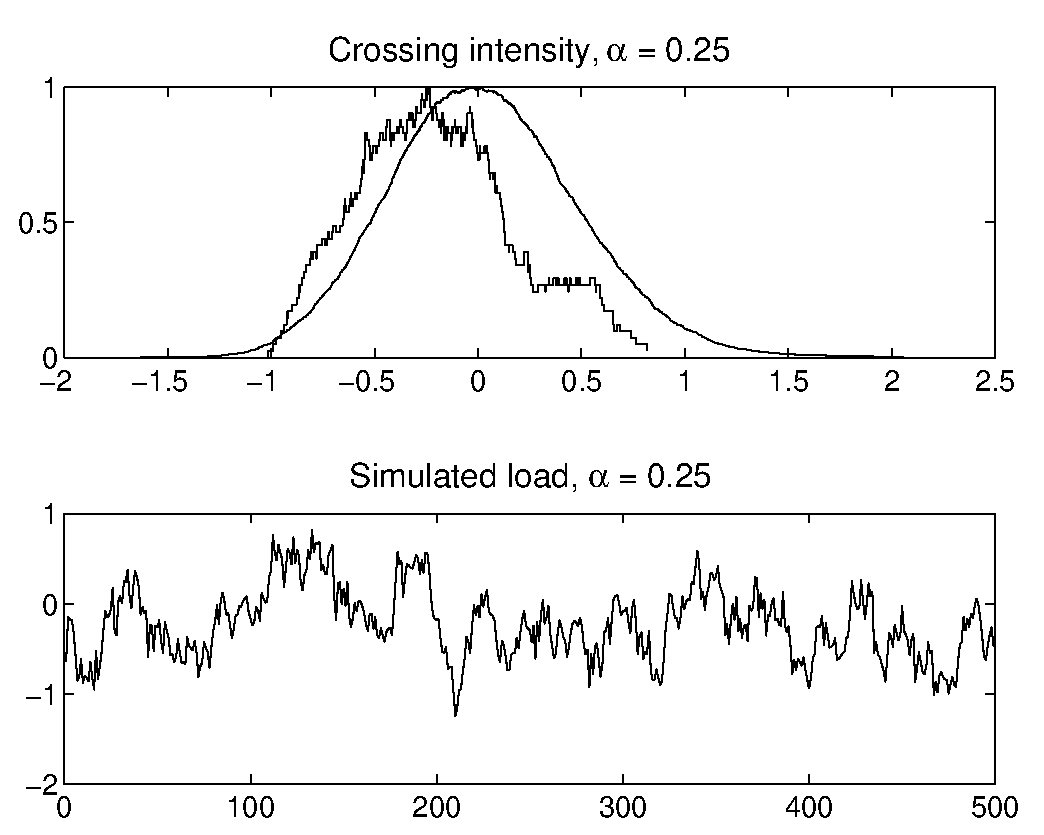
\includegraphics[width=\defwidth]{fatigue_14_25} \hspace{5mm}
  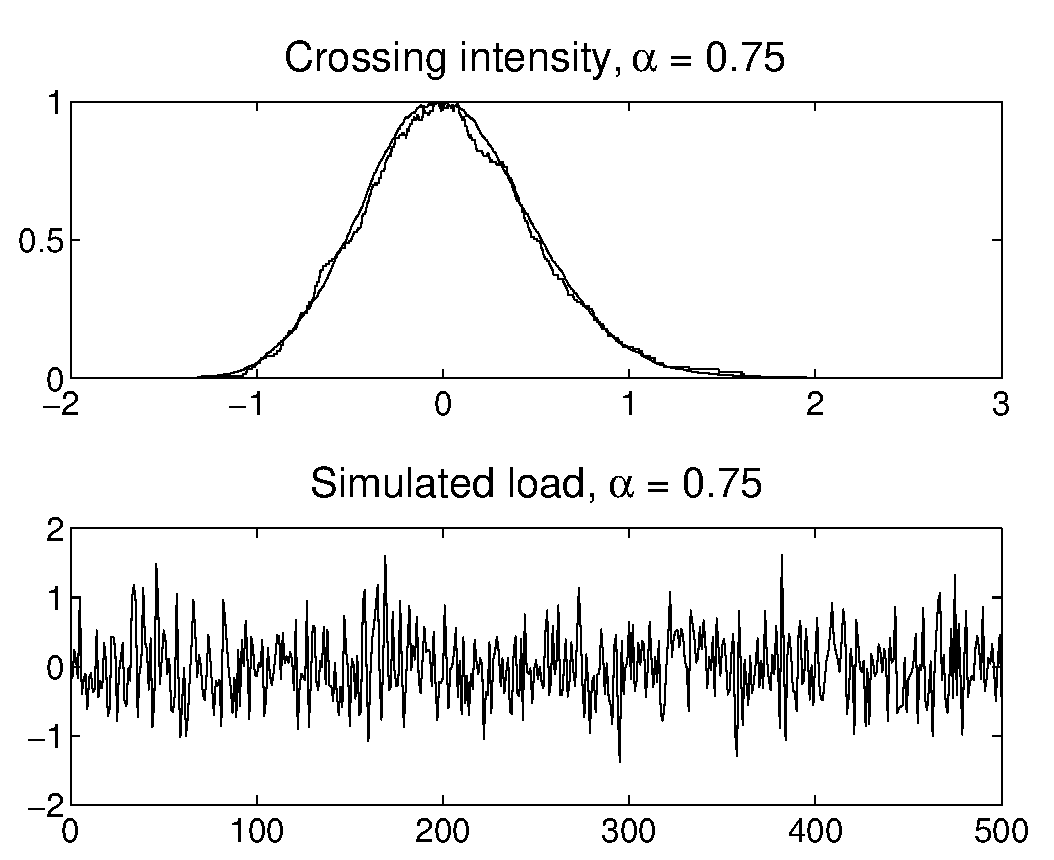
\includegraphics[width=\defwidth]{fatigue_14_75}
\vspace{-3mm}
\caption[Target and obtained crossing spectrum for simulated process]{
Upper figures show target crossing spectrum (smooth curve)
  and obtained spectrum (wiggled curve) for simulated process shown in
  lower figures. Irregularity factor: left $\alpha=0.25$, right
  $\alpha=0.75$.}
\label{fig_wafo_6.9}
\end{figure}


%\subsubsection{Simulation from rainflow structure}
%\label{rainflowsimulation}
%
%The routine {\tt rfm2dtp} generates a sequence of turning points
%from a rainflow matrix, and is an inverse routine to {\tt dtp2rfm}.
%The rainflow count of the output will be similar, but usually now exactly
%equal, to the input rainflow matrix. An example is given by the following
%command sequence. \index[xentr]{cycle analysis|)}\index[xcmds]{{\tt rfm2dtp}}
%{\small\begin{verbatim}
%      clf
%      x=load('sea.dat');
%      param = [-2 2 64]; n=param(3);
%      dtp0 = dat2dtp(param,x(:,2));
%      [RFM,RFM0,res0] = dtp2rfm(dtp0,n);
%      dtp = rfm2dtp(RFM0,res0);
%      plot(1:length(dtp0),dtp0,'b',1:length(dtp),dtp,'r')
%      RFMs=dtp2rfm(dtp,n);
%      max(max(abs(RFMs-RFM)))
%\end{verbatim}}
%Here, the rainflow matrix {\tt RFM} is identical to the matrix {\tt RFMs}, and
%the load sequence {\tt dtp} has the same length as the original data sequence
%{\tt sea.dat}.
%
%To simulate a new load sequence with the rainflow matrix {\tt RFM}
%one can use the following commands with {\tt mctpsim}:
%{\small\begin{verbatim}
%      clf
%      F = arfm2mctp(RFM);
%      xs = mctpsim(F,5000);
%      dtps = dat2dtp(param,xs);
%      RFMs2 = dtp2rfm(dtps);
%      u_levels=levels(param);
%      cmatplot(u_levels,u_levels,{RFM RFMs2},3)
%\end{verbatim}}
%\end{comment}

\section{Fatigue damage and fatigue
life distribution}\label{sec:damageintensity}
\index[xentr]{fatigue|(}

\subsection{Introduction}\label{sec:fatigueintroduction}
We shall now give a more detailed account of how
\progname{} can be used to estimate
and bound the fatigue life distribution under random loading.
%%%%%%%%%%%%%%%%%%%%%%%%%%%%%%%%%%%%%%%%%%%%%%%
% Level Crossings
%%%%%%%%%%%%%%%%%%%%%%%%%%%%%%%%%%%%%%%%%%%%%%%
The basic assumptions are the W{\" o}hler curve Eq.~(\ref{eq:SNmodel})
and the Palmgren-Miner damage accumulation rule Eq.~(\ref{eq:Damage}),
\index[xentr]{fatigue!life}\index[xentr]{fatigue!damage}\index[xentr]{damage}
\index[xentr]{W{\"o}hler curve}
\begin{eqnarray} %\label{SNmodel}
N(s)&=&\left\{ \begin{array}{c@{\quad}l}
K^{-1} s^{-\beta}, & s> s_{\infty},\\
\infty, & s\le s_{\infty},\end{array}\right.\label{eq:W} \\[0.6em]
  D(t)&=&\sum_{t_k\le t}\frac{1}{N(s_k)}=K\sum_{t_k\le
  t}s_k^\beta=K D_\beta(t). \label{eq:PM}
\end{eqnarray}
Here $N(s)$ is the expected fatigue life from constant amplitude test with
amplitude $s$, and $D(t)$ is the total damage at time $t$ caused by variable
amplitude cycles $s_k$, completed before time $t$.
The damage intensity $d_\beta = D(t)/t$ for large $t$ is the amount of
damage per time unit.

Most information is contained in the cycle amplitude distribution,
in particular in
the rainflow cycles, in which case (\ref{eq:PM}) becomes,
$$
  D(t) = \sum_{t_k\le t} \frac{1}{N_{s_k}}
  = K \sum_{t_k\le t} \left(S_k^{\rfc}\right)^{\beta}, \qquad
  S_k^{\rfc} = \left(M_k-m_k^{\rfc}\right)/2.
$$

The rainflow cycle count {\tt RFC} can be directly used for prediction of
expected fatigue life. The expression Eq.~(\ref{eq:fatiguelifetime}) gives the
expected time to fatigue failure in terms of the material constant $\epsilon$
and the expected damage $d_\beta$ per time unit. The parameters $\epsilon$ and
$\beta$ can be estimated from an S-N curve. In the examples here we will use
$\epsilon=5.5\cdot10^{-10}$, $\beta=3.2$;
see Section~\ref{sec:estimationofSNcurve}.
 % and $\sigma^2_K=0.06$.
For our sea load \verb+xx_sea+, the computations go directly from the
rainflow cycles as follows.
{\small\begin{verbatim}
      beta=3.2; gam=5.5E-10; T_sea=xx_sea(end,1)-xx_sea(1,1);
      d_beta=cc2dam(RFC_sea,beta)/T_sea;
      time_fail=1/gam/d_beta/3600
\end{verbatim}}
\noindent
giving the time to failure  {\tt 5.9693e+006} when time to
failure is counted in hours (= 3600 sec).
Obviously, this load causes little damage to the material with the
specified properties, since the failure time is almost 700 years --
of course, the sea wave data is not a fatigue load sequence, so the example is
meaningless from a fatigue point of view.

\subsection{Level Crossings}
\label{sec:levelcrossings}\index[xentr]{level crossing}
We have in Section~\ref{sec:crossingrainflowsimulation} seen how the crossing
intensity contains information about the load sequence and how it can be used
for simulation. We shall now investigate the relation between the crossing
intensity, the rainflow cycles, and the expected fatigue life.

We use the Markov model from Section~\ref{sec:simulationmarkov}
for the sequence of turning points as an example.
First we go from the rainflow matrix to the crossing
intensity.\index[xentr]{crossing intensity!calculation from rainflow matrix}
{\small\begin{verbatim}
      mu_markov = cmat2lc(param_m,Grfc_markov);
      muObs_markov = cmat2lc(param_m,Frfc_markov/(T_markov/2));
      plot(mu_markov(:,1),mu_markov(:,2),...
         muObs_markov(:,1),muObs_markov(:,2),'--')
      title('Theoretical and observed crossing intensity ')
\end{verbatim}}
The plot in Figure~\ref{fig_wafo_6.10} compares the
theoretical upcrossing intensity \verb+mu_markov+
with the observed upcrossing intensity \verb+muObs_markov+, as calculated
from the theoretical and observed rainflow matrices, respectively.

\begin{figure}
\centering
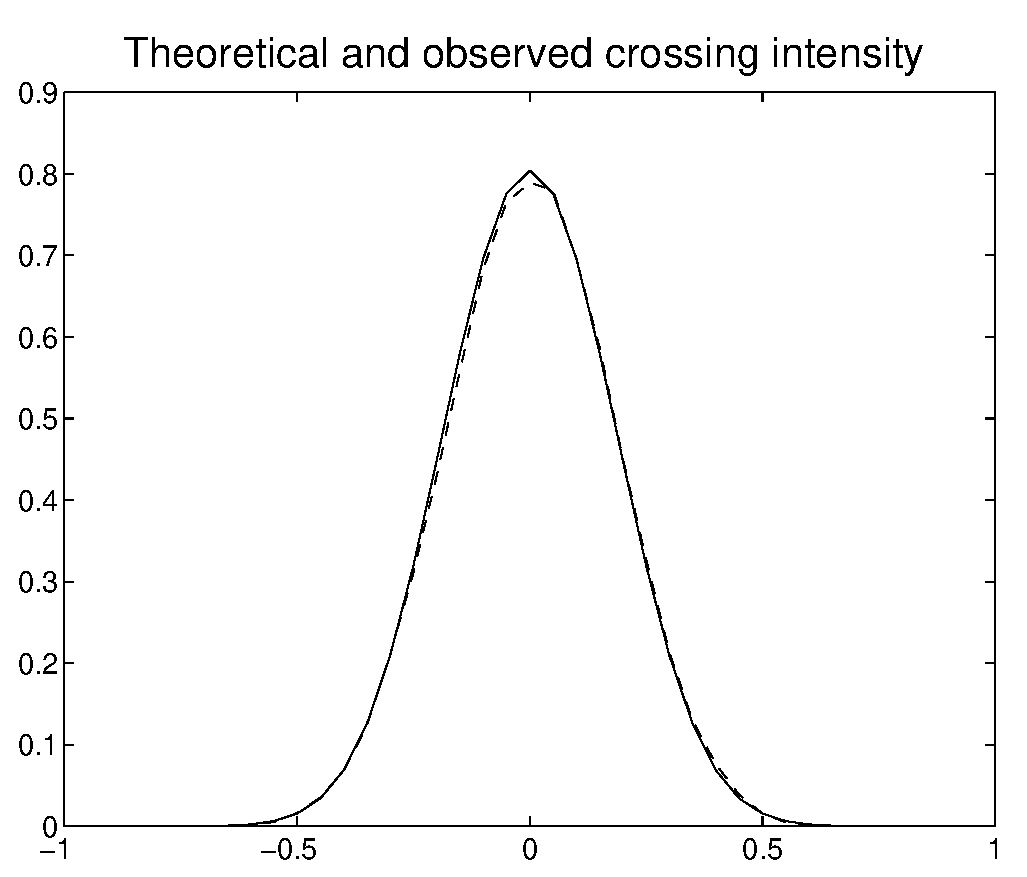
\includegraphics[width=\narrowfigwidth]{fatigue_15}
\vspace{-3mm}
\caption[Crossing intensity from Markov and observed rainflow matrix]
{Crossing intensity as calculated from the Markov observed rainflow matrix
(solid curve) and from the observed rainflow matrix (dashed curve).}
\label{fig_wafo_6.10}
\end{figure}

%%%%%%%%%%%%%%%%%%%%%%%%%%%%%%%%%%%%%%%%%%%%%%%
% Damage
%%%%%%%%%%%%%%%%%%%%%%%%%%%%%%%%%%%%%%%%%%%%%%%

\subsection{Damage}\index[xentr]{damage}
\label{sec:damage}
The \progname{} toolbox contains a number of routines to compute and bound
the damage, as defined by (\ref{eq:PM}), inflicted by a load sequence.
The most important routines are {\tt cc2dam}\index[xcmds]{{\tt cc2dam}}
and {\tt cmat2dam}\index[xcmds]{{\tt cmat2dam}}, which
give the total damage from a cycle count and from a cycle matrix,
respectively. More detailed information is given by
{\tt cmat2dmat}\index[xcmds]{{\tt cmat2dmat}},
which gives a damage matrix, separated for each cycle, from a cycle
matrix. An upper bound for total damage from level crossings is
given by {\tt lc2dplus}\index[xcmds]{{\tt lc2dplus}}.

%    snplot      - Plots S-N data and estimates parameters. (FAT)
%  o sphdam      - Calculates spherical damage for a 3-D load. (FAT)
%    ftf         - Calculates fatigue failure time distribution. (FAT)
%  o damint      - Calculates damage intensity from counting distribution. (FAT)
%  o down2cc     - Calculates the most damaging cycle count given crossings.(FAT)
%  o roadspec    - Road spectrum. (FAT)

We first calculate the damage by the routines {\tt cc2dam}
for a cycle count (e.g.\ rainflow cycles) and {\tt cmat2dam} for
a cycle matrix (e.g.\ rainflow matrix).
{\small\begin{verbatim}
      beta = 4;
      Dam_markov = cmat2dam(param_m,Grfc_markov,beta)
      DamObs1_markov = ...
         cc2dam(u_markov(RFC_markov),beta)/(T_markov/2)
      DamObs2_markov = ...
         cmat2dam(param_m,Frfc_markov,beta)/(T_markov/2)
\end{verbatim}}
Here, \verb+Dam_markov+ is the theoretical damage per cycle in the
assumed Markov chain of turning points, while \verb+DamObs1+ and
\verb+DamObs2+ give the observed damage per cycle, calculated
from the cycle count and from the rainflow matrix, respectively.
For this model the result should be
\verb+Dam_markov = 0.0073+ for the theoretical damage and very
close to this value for the simulated series.

The damage matrix is calculated by {\tt cmat2dmat}. It shows how the
damage is distributed among the different cycles as illustrated in
Figure~\ref{fig_wafo_6.11}. The sum of all the
elements in the damage matrix gives the total damage.
{\small\begin{verbatim}
      Dmat_markov = cmat2dmat(param_m,Grfc_markov,beta);
      DmatObs_markov = cmat2dmat(param_m,...
                                Frfc_markov,beta)/(T_markov/2);}
      subplot(121), cmatplot(u_markov,u_markov,Dmat_markov,4)
      title('Theoretical damage matrix')
      subplot(122), cmatplot(u_markov,u_markov,DmatObs_markov,4)
      title('Observed damage matrix')
      sum(sum(Dmat_markov))
      sum(sum(DmatObs_markov))
\end{verbatim}}

\begin{figure}
\centering
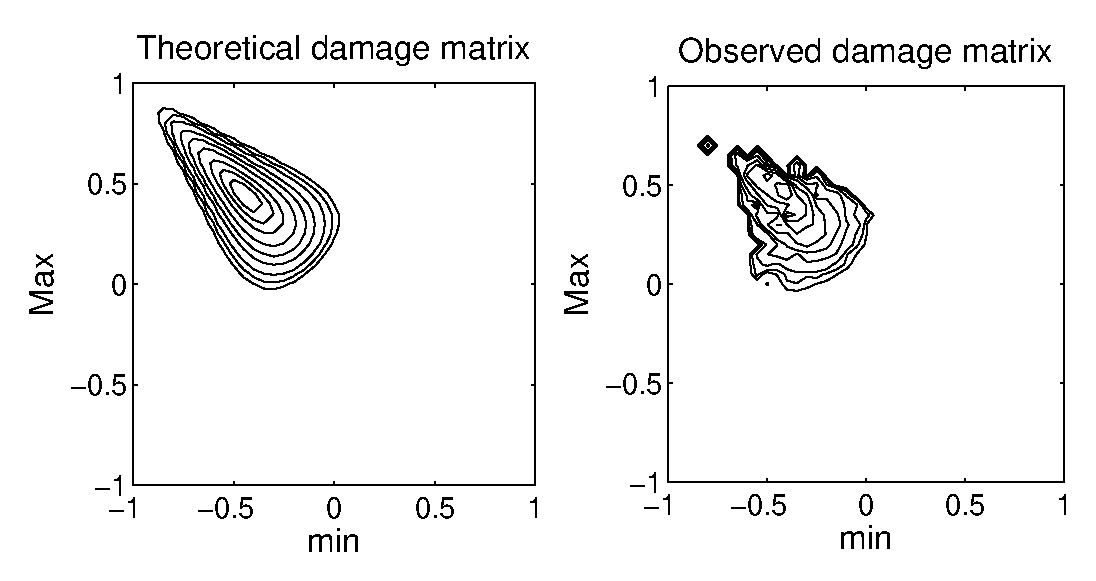
\includegraphics[width=\onefigwidth]{fatigue_16}
\vspace{-3mm}
\caption[Distribution of damage from RFC cycles]
{Distribution of damage from different RFC cycles,
from calculated theoretical and from observed rainflow matrix.}
\label{fig_wafo_6.11}
\end{figure}

It is possible to calculate an upper bound on the damage intensity
from the crossing intensity only, without using the rainflow cycles.
This is done by the routine {\tt lc2dplus}, which works
on any theoretical or observed crossing intensity function.
{\small\begin{verbatim}
      Damplus_markov = lc2dplus(mu_markov,beta)
\end{verbatim}}

\subsection{Estimation of S-N curve}\label{sec:estimationofSNcurve}
\index[xentr]{S-N curve!estimation of}

\progname{} contains routines for computation of parameters in the
basic S-N curve (\ref{eq:SNmodel}), for the relation between the load cycle
amplitude $s$ and the fatigue life $N(s)$ in fixed amplitude tests,
defined by (\ref{eq:W}).
%        \begin{equation} %\label{SNmodel}
%        N(s)=\left\{ \begin{array}{c@{\quad}l}
%        K^{-1} s^{-\beta} & s> s_{\infty},\\
%        \infty & s\le s_{\infty},\end{array}\right.
%        \end{equation}
The variation of the material dependent variable $K$ is often
taken to be random with a lognormal distribution,
$$
K = E \epsilon ^{-1},
$$
where $\epsilon$ is a fixed parameter, depending on material,
and $\ln E$ has a normal distribution with mean $0$ and
standard deviation $\sigma _E$. Thus, there are three
parameters, $\epsilon$, $\beta$, $\sigma _E$,
to be estimated from an S-N experiment.
Taking logarithms in (\ref{eq:SNmodel})
the problem turns into a standard regression problem,
$$
\ln N(s) = - \ln E - \ln \epsilon - \beta \ln s,
$$
in which the parameters can easily be estimated.

The \progname{} toolbox contains a data set {\tt sn.dat}
with fatigue lives from 40 experiments with
$s$ = 10, 15, 20, 25, and 30 MPa, stored in a variable \verb+N+,
in groups of five.
The estimation routine is called {\tt snplot}\index[xcmds]{{\tt snplot}},
which performs both estimation and
plotting; see {\tt help snplot}.

First load SN-data and plot in log-log scale.
{\small\begin{verbatim}
      SN = load('sn.dat');
      s = SN(:,1); N = SN(:,2);
      loglog(N,s,'o'), axis([0 14e5 10 30])
\end{verbatim}}
To further check the assumptions of the S-N-model
we plot the results for each $s$-level separately on normal
probability paper. As seen from Figure~\ref{fig_wafo_6.14}
the assumptions seem acceptable since the data fall on
almost parallel straight lines.
{\small\begin{verbatim}
      plotnorm(reshape(log(N),8,5))
\end{verbatim}}

\begin{figure}
\centering
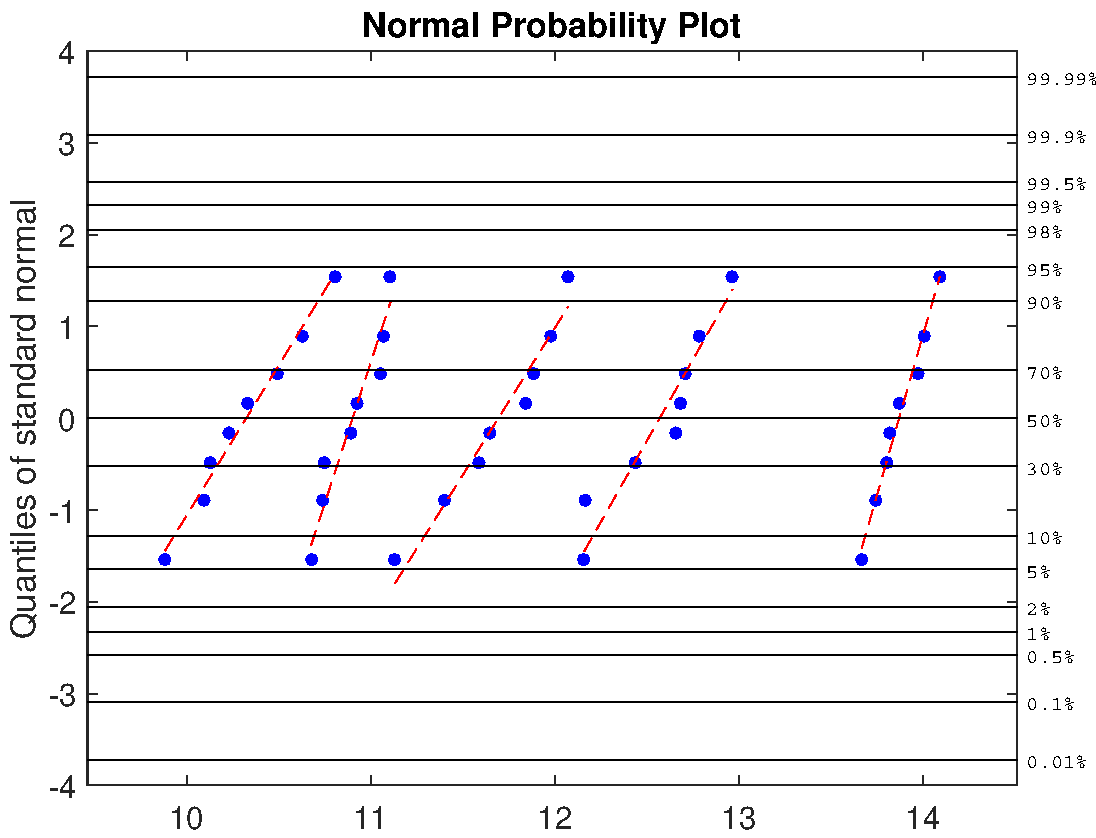
\includegraphics[width=\narrowfigwidth]{fatigue_17_2017}
\vspace{-3mm}
\caption[Check of S-N-model on normal probability paper]
{Check of S-N-model on normal probability paper.}
\label{fig_wafo_6.14}
\end{figure}

The estimation is performed and fitted lines plotted in
Figure~\ref{fig_wafo_6.15}, with linear and log-log plotting scales:
{\small\begin{verbatim}
      [e0,beta0,s20] = snplot(s,N,12);
      title('S-N-data with estimated N(s)')
\end{verbatim}}
\noindent gives linear scale and
{\small\begin{verbatim}
      [e0,beta0,s20] = snplot(s,N,14);
      title('S-N-data with estimated N(s)')
\end{verbatim}}
\noindent gives log-log scales.

\begin{figure}
\centering
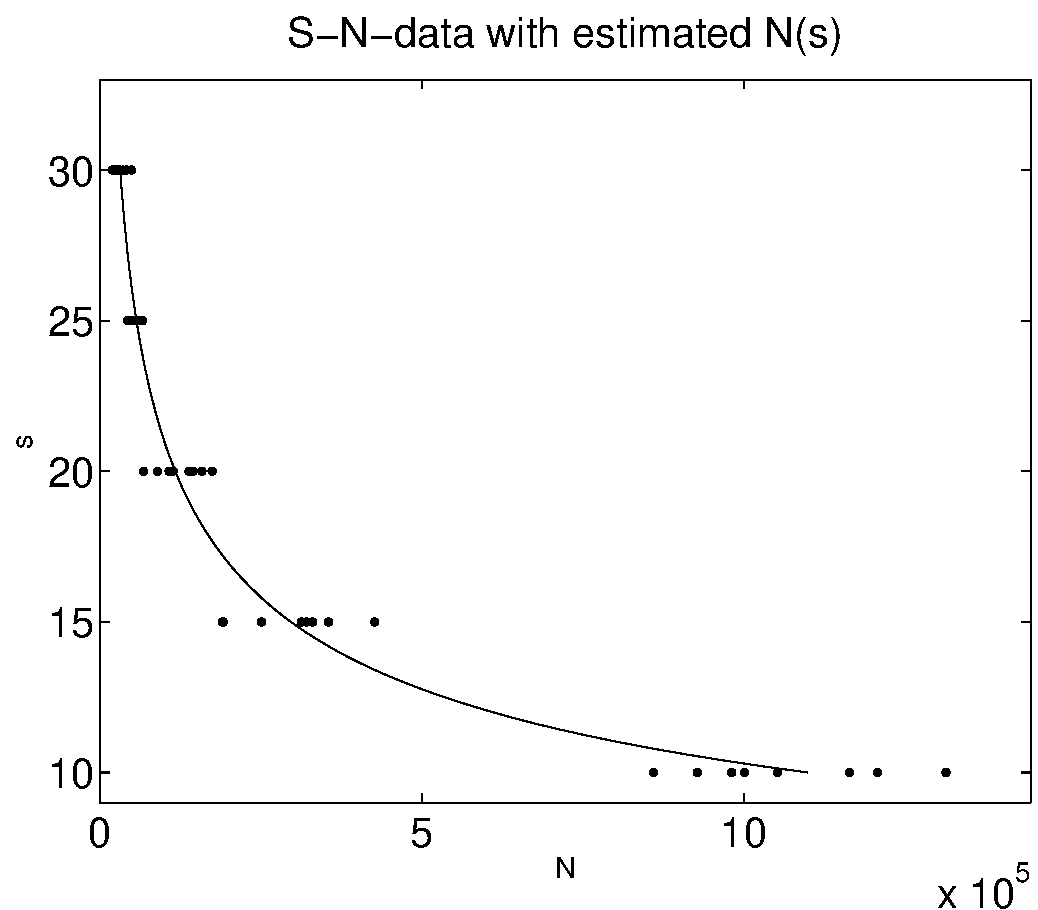
\includegraphics[width=\defwidth]{fatigue_18a}%
\hspace{5mm}
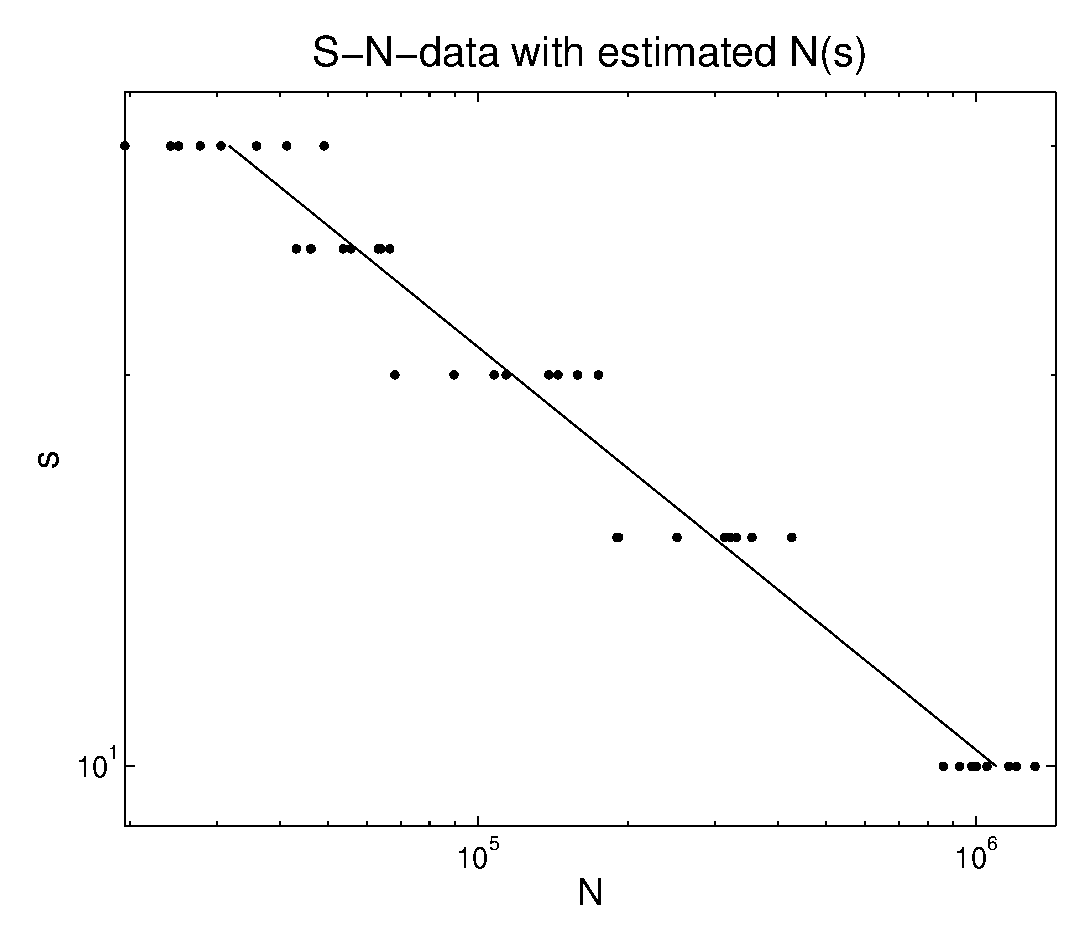
\includegraphics[width=\defwidth]{fatigue_18b}
\vspace{-3mm}
\caption[Estimation of S-N-model on linear and log-log scale]
{Estimation of S-N-model on linear and log-log scale.}
\label{fig_wafo_6.15}
\end{figure}

\subsection{From S-N-curve to fatigue life distribution}
\label{sec:fatiguelifedistribution}\index[xentr]{fatigue!life!distribution}

The Palmgren-Miner hypothesis states that fatigue failure occurs
when the accumulated damage exceeds one, $D(t) > 1$.
Thus, if the fatigue failure time is denoted by $T_f$, then
$$
\pr(T_f \leq t) = \pr(D(t) \geq 1) = \pr(K \leq \epsilon D_\beta (t)).
$$
Here $K=E^{-1}\epsilon$ takes care of the uncertainty in the material.
In the previous section we used and estimated a lognormal distribution
for the variation of $K$ around $\epsilon$, when we assumed
that $\ln K = \ln \epsilon - \ln E$ is normal with
mean $\ln \epsilon$ and standard deviation $\sigma _E$.

The cycle sum $D_\beta(t)$ is the sum of a large number of damage
terms, only dependent on the cycles. For loads with short memory
one can assume that $D_\beta(t)$ is approximately normal,
$$
D_\beta(t) \approx N(d_\beta t,\, \sigma_\beta ^2 \,t),
$$
where
$$
d_\beta = \lim _{t \to \infty} \frac{D_\beta (t)}{t} \qquad \mbox{and} \qquad
\sigma_\beta ^2 =  \lim _{t \to \infty} \frac{V(D_\beta (t))}{t}.
$$

Thus the fatigue life distribution can be computed by combining the lognormal
distribution for $K$ with the normal distribution
for $D_\beta (t)$. Denoting the standard normal density and distribution functions
by $\phi(x)$ and $\Phi(x)$, respectively, an approximate  explicit expression
for the failure probability within time $t$ is
\begin{equation}
\pr(T^f \leq t) \approx \int_{-\infty}^\infty
\Phi \left(
\frac{\ln \epsilon + \ln d_\beta t +
\ln (1 + \frac{\sigma_\beta}{d_\beta \sqrt{t}}z)}{\sigma_E}
\right) \phi (z) \,dz.
\label{eq:failuretimedistribution}
\end{equation}

We have already estimated the material dependent
parameters $\epsilon$ \verb+= e0+,
$\beta$ \verb+= beta0+, and $\sigma _E ^2$ \verb+= s20+,
in the S-N data, so we need the damage intensity $d_\beta$ and its
variability $\sigma _\beta$ for the acting load.

We first investigate the effect of uncertainty in the $\beta$-estimate.
{\small\begin{verbatim}
      beta = 3:0.1:8;
      DRFC = cc2dam(RFC_sea,beta);
      dRFC = DRFC/T_sea;
      plot(beta,dRFC), axis([3 8 0 0.25])
      title('Damage intensity as function of \beta')
\end{verbatim}}
\noindent
The plot in Figure~\ref{fig_wafo_6.17} shows the increase in damage with
increasing $\beta$.
\begin{figure}[tbh]
\centering
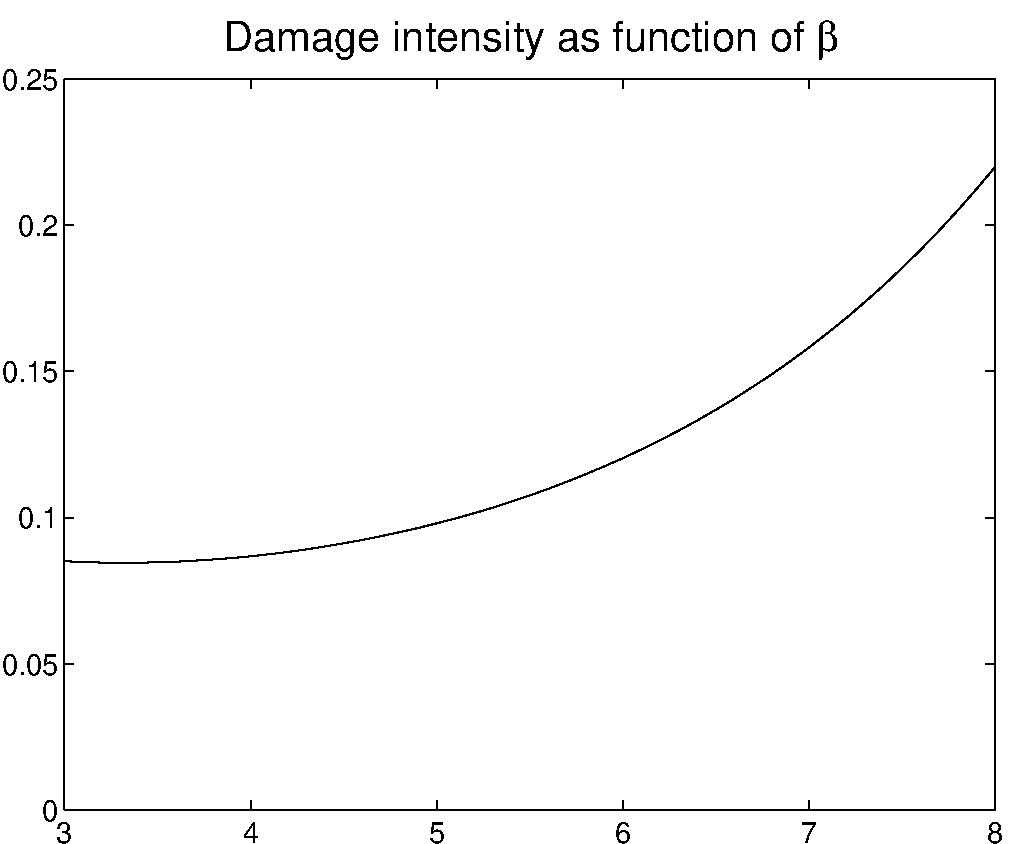
\includegraphics[width=\narrowfigwidth]{fatigue_19}
\vspace{-3mm}
\caption[Increasing damage intensity from sea-load with increasing $\beta$]
{Increasing damage intensity from sea-load with increasing $\beta$.}
\label{fig_wafo_6.17}
\end{figure}

Next, we shall see how the load variability affects the fatigue life.
We use three different values for $\sigma _\beta ^2$, namely $0$, $0.5$,
and  $5$. With \verb+beta0+, \verb+e0+, \verb+s20+ estimated in
Section~\ref{sec:estimationofSNcurve}, we compute and plot the following three
possible fatigue life distributions.
{\small\begin{verbatim}
      dam0 = cc2dam(RFC_sea,beta0)/T_sea;
      [t0,F0] = ftf(e0,dam0,s20,0.5,1);
      [t1,F1] = ftf(e0,dam0,s20,0,1);
      [t2,F2] = ftf(e0,dam0,s20,5,1);
      plot(t0,F0,t1,F1,t2,F2)
\end{verbatim}}
\noindent
Here, the fourth parameter is the value of $\sigma _\beta^2$ used in the
computation; see \verb+help ftf+.

\begin{figure}[bth]
\centering
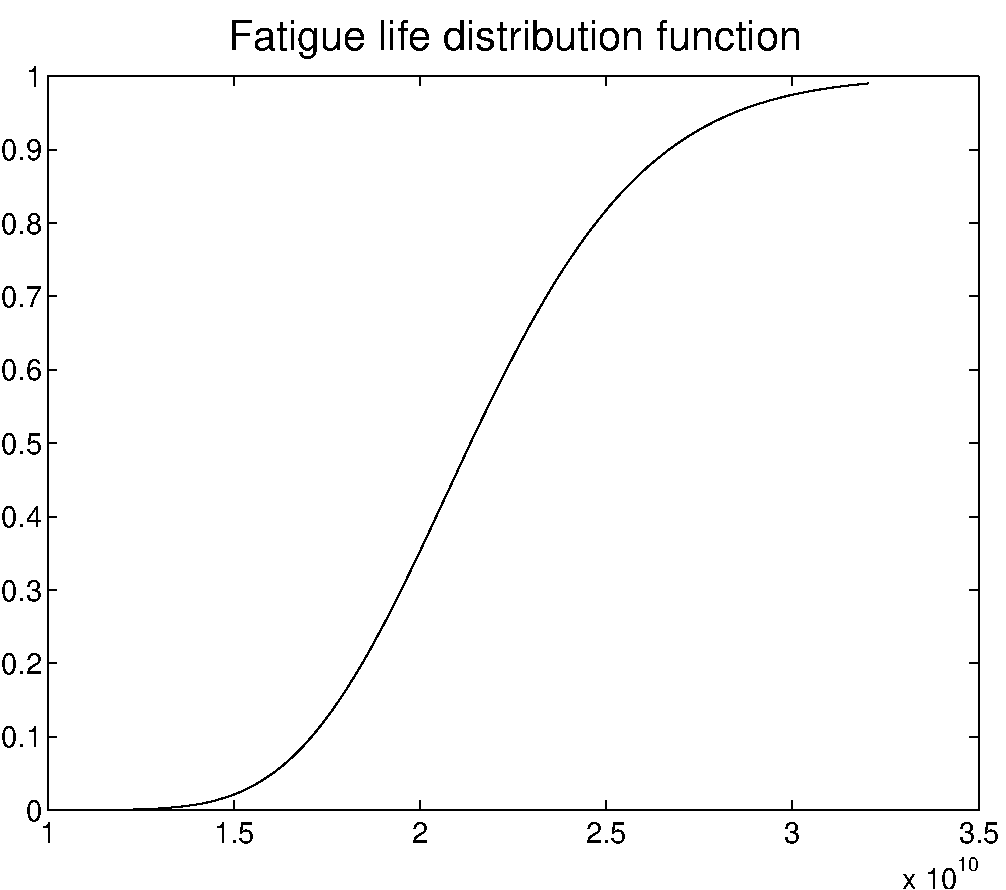
\includegraphics[width=\narrowfigwidth]{fatigue_20}
\vspace{-3mm}
\caption[Fatigue life distribution with sea load]
{Fatigue life distribution with sea load.}
\label{fatigue_20}
\end{figure}

The resulting fatigue life distribution function
is shown in Figure~\ref{fatigue_20}.
As seen, the curves are identical, indicating that the correct value of
$\sigma _\beta ^2$ is not important for such small $\epsilon$-values
as are at hand here. Hence, one can use $\sigma _\beta ^2 = 0$, and
assume that the damage accumulation process is proportional to time.

\subsection{Fatigue analysis of complex loads}\label{sec:complexloads}
Loads which cause fatigue are rarely of the homogeneous and stationary
character as the loads used in the previous sections. On the contrary,
typical load characteristics often change their value during the life time
of a structure, for example, load spectra on an airplane part have
very different fatigue properties during the different stages of an
air mission. Marin loads on a ship are quite different during 
loading and unloading, compared to a loaded ocean voyage, and the
same holds for any road vehicle.

The \progname{} toolbox
can be used to analyse also loads of complex structure
and we shall illustrate some of these capabilities in this section.
To be eligible for \progname-analysis, the loads have to have a
piecewise stationary character, for example the mean level or the standard
deviation may take two distinct levels and change abruptly,
or the frequency content can alternate between
two modes, one irregular and one more regular. Such processes are called
{\it switching processes}\index[xentr]{switching load}.
A flexible family of switching loads are those
where the change between the different stationary states is governed by
a Markov chain. \progname{}
contains a special package of routines for analysis
of such switching Markov loads, based on methods by Johannesson,  
\cite{Johannesson1998Rainflow,Johannesson1999Rainflow}.

In the following example the load alternates between two different
mean levels, corresponding to one heavy-load state (1) and one light-load
state (2). In Figure~\ref{fatigue_21} the observed load is shown
in the upper part. The alternating curve in the lower part shows
the switches between the two states.
\begin{figure}[bth]
  \centering
    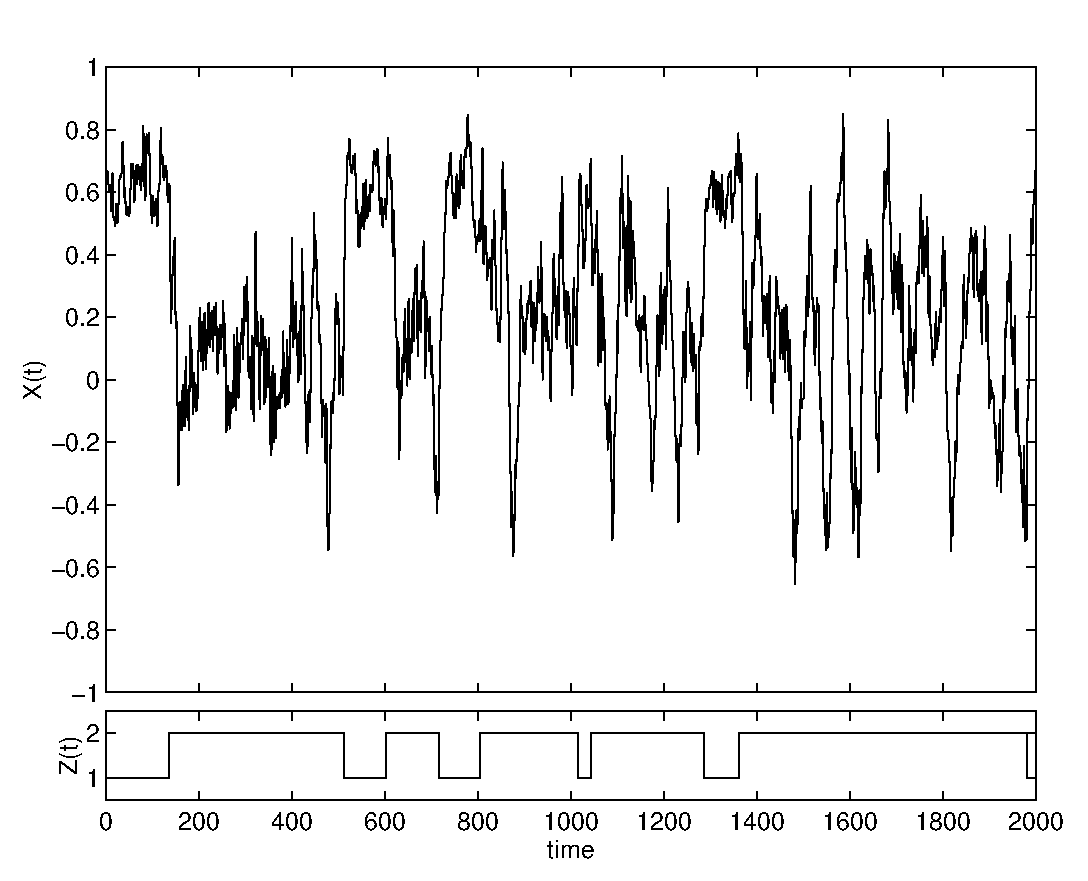
\includegraphics[width=\narrowfigwidth]{FigEx2SamplePath}
\vspace{-3mm}
\caption[Simulated switching load with two states]
{Simulated switching load with two states. Upper graph shows the
load, and the states are indicated in the lower graph.}
\label{fatigue_21}
\end{figure}

As long as the load is in one of the states, the rainflow cycles are
made up of alternations between turning points belonging only
to that part of the load. When the state changes there is introduced
extra rainflow cycles with larger amplitudes. These extra cycles
can be seen in the total rainflow matrix, shown in Figure~\ref{fatigue_22}.
The two large groups of cycles around (min,max) = (0.5, 0.75) and
(min,max) = (0, 0) come from states (1) and (2), respectively.
The contribution from the switching is seen in the small
assembly of cycles around (min,max) = (-0.5, 1).

More details on how to analyse and model switching loads can be found in
\cite{Johannesson1997Matlab}.%,Johannesson97.M1}.

%\newpage
\begin{figure}[tbh]
\subfigure[ Rainflow matrix]{%
\begin{minipage}[b]{0.5\textwidth}%
\centering 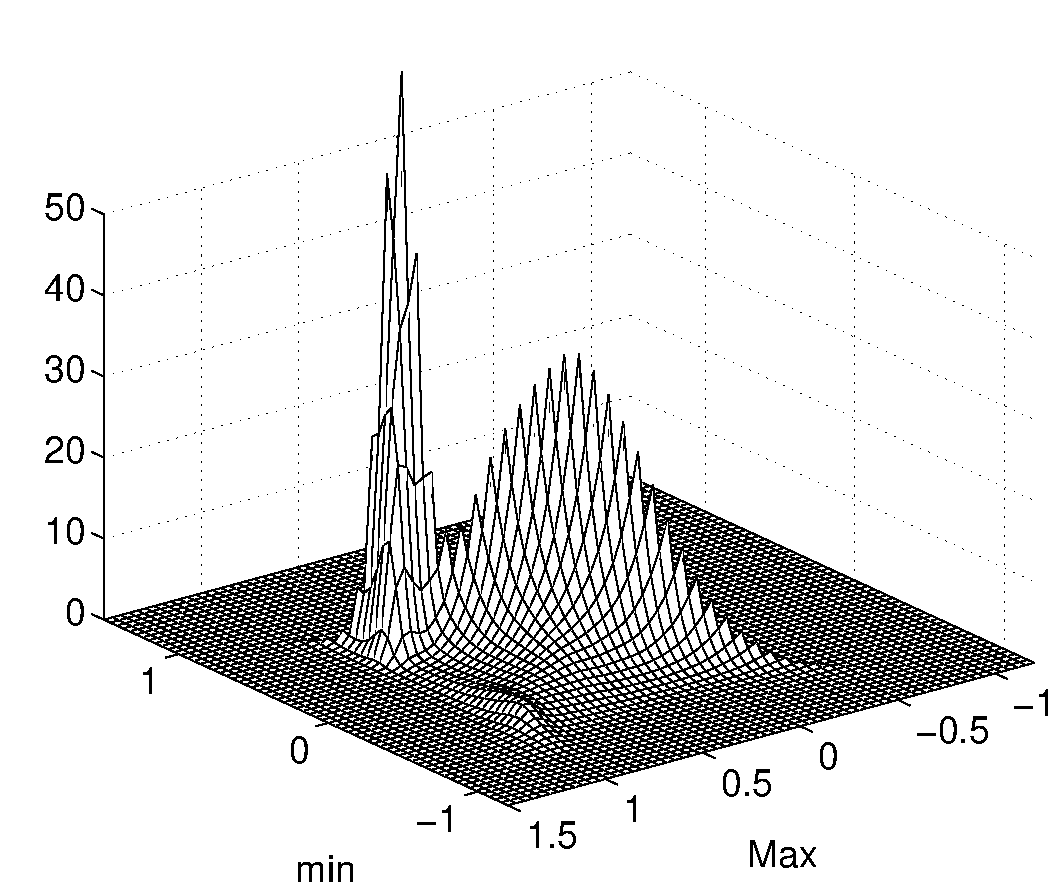
\includegraphics[width=\defwidth]{FigEx2RFCint3D}
\end{minipage}}%
\hfill
\subfigure[Rainflow matrix]{%
\begin{minipage}[b]{0.5\textwidth}%
\centering 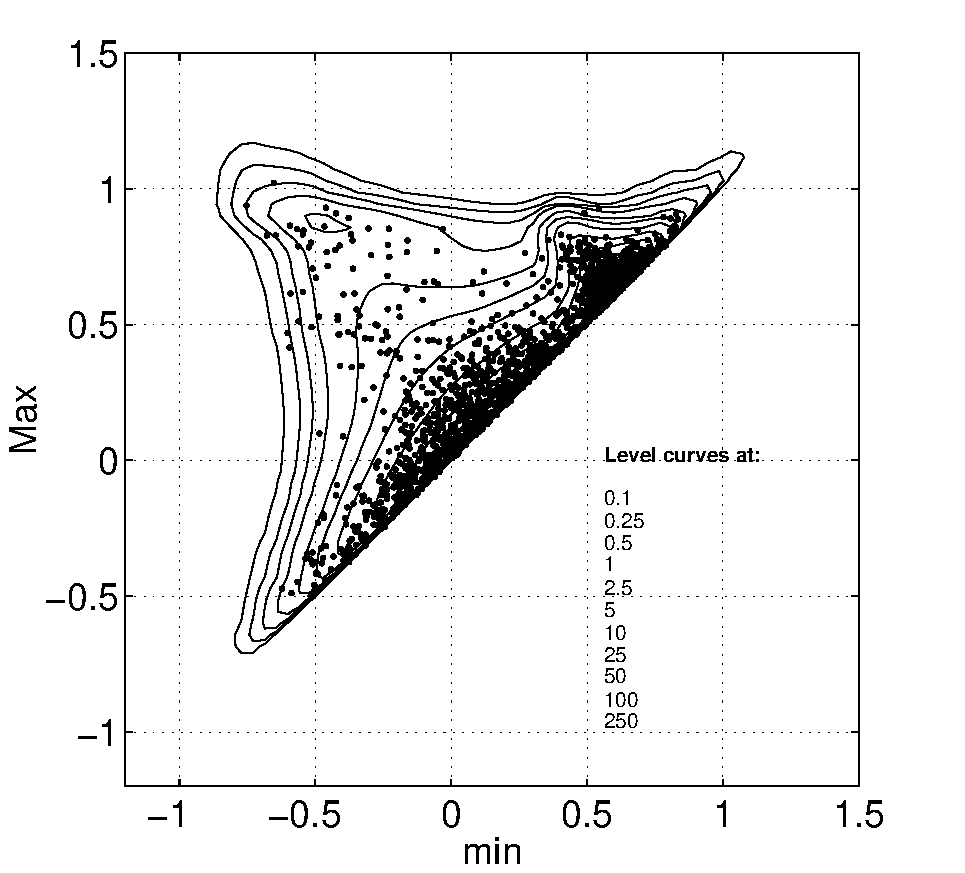
\includegraphics[width=\defwidth]{FigEx2RFCintCC}
\end{minipage}}
\vspace{-3mm}
\caption[3D-plot and isolines of calculated rainflow matrix]
{3D-plot (left) and isolines (right) of calculated rainflow matrix
for switching load in Figure~\ref{fatigue_21}. The dots in the right figure
are the observed rainflow cycles.}
\label{fatigue_22}
\end{figure}
\index[xentr]{fatigue|)}%\index[xentr]{random fatigue|see fatigue}

%\bibliography{wafoBibliography}


%%% Local Variables:
%%% mode: latex
%%% TeX-master: "wafomanual"
%%% End:
